% !TEX program = xelatex
\documentclass[12pt,ngerman]{scrartcl}
\usepackage{microtype}
\usepackage{fontspec}
\setmainfont{Times New Roman}
\setkomafont{disposition}{\rmfamily\bfseries}
\setkomafont{section}{\normalsize\bfseries}
\setkomafont{subsection}{\normalsize\bfseries}
\setkomafont{subsubsection}{\normalsize\bfseries}
\setkomafont{paragraph}{\normalsize\bfseries}
\setkomafont{subparagraph}{\normalsize\bfseries}
\setkomafont{caption}{\normalsize}
\setkomafont{captionlabel}{\normalsize\bfseries}
\setkomafont{title}{\rmfamily\bfseries\normalsize}
\setlength{\parskip}{\medskipamount}
\setlength{\parindent}{0pt}
\usepackage{babel}
\usepackage{float}
\usepackage{amsmath}
\usepackage{amstext}
\usepackage{varioref}
\usepackage[unicode=true,pdfusetitle,
bookmarks=true,bookmarksnumbered=false,bookmarksopen=false, breaklinks=false,pdfborder={0 0 0},backref=false,colorlinks=false] {hyperref}
\usepackage{graphicx}
\usepackage{setspace}
\usepackage{cleveref}
\usepackage{icomma}
\usepackage{booktabs}
\usepackage{blindtext}
\usepackage{outlines}
\usepackage{graphicx}
\usepackage{titling}
\usepackage{csquotes}
\usepackage{lscape}
\usepackage{longtable}
\usepackage{array}
\MakeOuterQuote{"}
\usepackage[
backend=biber,
style=apa,
sorting=nyt
]{biblatex}
\DeclareLanguageMapping{ngerman}{ngerman-apa}

% % % % % % % % % % % % % % % % % % % % %
% Zeilenabstand
\usepackage{setspace}
\onehalfspacing % 1,5-facher Zeilenabstand für den gesamten Text

\widowpenalties=3 10000 10000 150
% Aktiviert Blocksatz:
\usepackage{ragged2e}
\justifying

% Seitenränder
\usepackage[
top=2.5cm,    % Oberer Rand
bottom=2cm,   % Unterer Rand
left=2.5cm,   % Linker Rand
right=3.5cm   % Rechter Rand
]{geometry}



% Literatur
\addbibresource{literatur.bib}
% % % % % % % % % % % % % % % % % % % % %
\makeatletter
\begin{document}
	%%Hier alle Daten einfügen
\newcommand{\autorname}{Andrea Marsing}
\newcommand{\autormail}{andrea.marsing@uni-potsdam.de}
\newcommand{\autormatr}{831593}
\newcommand{\fak}{Wirtschafts- und Sozialwissenschaftliche Fakultät}
\newcommand{\lehrstuhl}{Professur für Internationale Beziehungen}
\newcommand{\lv}{Studying International Organizations}
\newcommand{\semester}{Sommersemester 2026}
\newcommand{\lp}{Dr. Andrea Knapp}
\newcommand{\arbtyp}{Hausarbeit}
\newcommand{\titel}{IMF-Konditionalität, UNSC und Dependenztheorie}

\title{\titel}
\author{\autorname}
	\begin{titlepage}
\vspace*{4cm}
\noindent\hspace*{\dimexpr(\paperwidth-\textwidth)/2-1in-\hoffset-\oddsidemargin\relax}
\begin{tabular}{@{}>{\centering\arraybackslash}p{\textwidth}@{}}
	\toprule
	\toprule[2pt]
	{\huge\bfseries \titel}\\[0.5em]
	{\Large \arbtyp}\\
	\bottomrule[2pt]
	\bottomrule
\end{tabular}
\vspace{3cm}
\centering{
}
\vspace{3cm}
\begin{center}
\begin{tabular}{@{}l l@{}}
\textit{Autor} & \Large \autorname\\
\textit{Fakultät} & \fak\\
\textit{Lehrstuhl} & \lehrstuhl\\
\textit{Lehrveranstaltung} & \lv\\
\textit{Semester} & \semester\\
\textit{Lehrperson} & \lp \\
\end{tabular}
\end{center}
\vfill

\includegraphics[width=2cm]{res/uni_potsdam_logo.pdf}

\end{titlepage}

\tableofcontents
\vfill
\hrule
\begin{center}\autorname~$\cdot$ \autormatr~$\cdot$ \href{mailto:\autormail}{\autormail}\end{center}
	\clearpage
	%\tableofcontents
% TODO: Klaeren, ob ein Inhaltsverzeichnis gefordert ist.
	\clearpage
	
	\section{Einleitung}
	\label{sec:einleitung}
	\noindent
	\textbf{Problemstellung:} Hier die zentrale Forschungsfrage, Relevanz und Ausgangslage der Arbeit eintragen.
% SLOT EI-1 — Problemstellung / Forschungsfrage (3-4 eigene Saetze)
% Muss enthalten: (a) IMF-Konditionalitaet praegt Politik im Globalen
% Sueden; (b) umkaempfte Frage: Ist die Strenge politisch ungleich
% verteilt? (Stone-Linie; DSV 2015 zeigen fuer 1992-2008 einen
% UNSC-"Rabatt" von rund 30 Prozent \parencite[121]{DreherPoliticsIMFConditionality2015});
% (c) Forschungsfrage: haelt dieser Befund ueber den Originalzeitraum
% hinaus? (d) Relevanz: Rueckkehr des IMF als Kreditgeber nach der
% Finanzkrise \parencite[545]{KentikelenisIMFConditionalityDevelopment2016}.
% SLOT EI-2 — Forschungsstand-Kurzabriss (2-3 eigene Saetze, optional)
% Drei Strassen: (1) Determinanten von IMF-Vergabe und Strenge
% \parencite{BarroIMFProgramsWho2005} (Auswahlmechanik) und Stone-Linie
% (Geopolitik); (2) Entwicklung der Konditionalitaet
% \parencite[545]{KentikelenisIMFConditionalityDevelopment2016};
% (3) DSV 2015 als Ausgangspunkt der eigenen Replikation.
	
	\medskip
	\textbf{Ziel der Arbeit:} Hier kurze Einordnung der Forschungsfrage, des Beitrags und der zentralen Hypothesen formulieren.
% SLOT EI-3 — Ziel und Beitrag (2-3 eigene Saetze)
% Muss enthalten: Replikation des DSV-Designs mit ERWEITERTem
% Zeitraum 1992-2023 bei identischer Messregel; Vorab-Kennzeichnung
% der Testhierarchie (H1/H2 konfirmatorisch, H3 explorativ, H4 nicht
% konfirmatorisch — Anti-HARKing); Kernbefund als Vorankuendigung:
% keine Evidenz fuer den UNSC-Effekt im erweiterten Zeitraum, der
% Effekt ist zeitlich in den 1990ern lokalisiert.
	
	\medskip
	\textbf{Aufbau der Arbeit:} Ein kurzer Absatz zur Gliederung in Theorie, Daten, Ergebnisse, Diskussion und Fazit.
% SLOT EI-4 — Aufbau (1 Absatz)
% Roten Faden sichtbar machen: Theorie (Konditionalitaet ->
% politische Oekonomie -> Dependenztheorie -> Hypothesen) -> Daten &
% Methodik (Phase-A-Validierung + Phase-B-Panel, Messregeln,
% Abweichungen vom Original) -> Ergebnisse (H1/H2 konfirmatorisch,
% H3/H4 explorativ) -> Diskussion (1990er-Befund, Limitationen,
% Ausblick) -> Fazit.
	
	\section{Theorie}
\label{sec:theorie}

		% Theorie-Teil der Hausarbeit
% ----------------------------------------------------------------------
% GERUEST-Konventionen (vor Abgabe alle Marker entfernen bzw. aufloesen):
%   SLOT  = hier fehlen eigene 2-4 Saetze zu der im Kommentar beschriebenen
%           Behauptung; Quellenangabe steht schon bereit.
%   NOTIZ = eigene Rohnotiz, noch nicht in Prosa verwandelt.
%   TODO  = Fundstelle (Seitenzahl) noch an der Quelle pruefen.
% Regel: Keine Aussage ohne \parencite, kein \parencite ohne gepruefte
% Fundstelle. Alle SLOT/NOTIZ/TODO muessen vor Abgabe verschwunden sein.

\subsection{Theoretischer Rahmen}

% ----------------------------------------------------------------------
% ABSATZ 1: Begriff und Mechanismus der Konditionalitaet
% (eigene Saetze vorhanden; Seitenzahlen pruefen)
% ----------------------------------------------------------------------
Konditionalität bezeichnet die vom IMF vorgeschriebenen Policy-Reformen \parencite[545]{KentikelenisIMFConditionalityDevelopment2016}.

\textcite{DreherPoliticsIMFConditionality2015} beschreiben Konditionalität als die Notwendigkeit von Regierungen, für den Erhalt notwendiger Kredite von der IMF vorgegebene Policy-Änderungen (Schließen von Haushaltsdefiziten, Erhöhung von Zinsraten, etc.) zu befolgen.

% SLOT 1 — Auszahlungsmechanismus (2-3 eigene Saetze)
% Behauptung: Vergabe und fortlaufende Auszahlung der Kredite sind an die
% Einhaltung der Bedingungen gekoppelt; UEberpruefung erfolgt regelmaessig
% (quartalsweise Reviews); Konditionalitaet ist deshalb kontinuierlich
% verhandelbar, nicht nur eine einmalige Vereinbarung.
% Quelle: \parencite[TODO]{DreherPoliticsIMFConditionality2015}
% NOTIZ (vorhandene Rohnotiz):
%   Die Vergabe und kontinuierliche Auszahlung von IMF-Krediten sind meist
%   daran gekoppelt, ob Regierungen bestimmten Policy-Bedingungen folgen,
%   die jedes Quartal überprüft werden. Diese Arrangements sind bekannt
%   für ihre strenge und kontroverse ökonomische Austerität.

% ----------------------------------------------------------------------
% ABSATZ 2: Politische Oekonomie der Konditionalitaet
% (eigene Saetze vorhanden; NOTIZ-Stueck unten einarbeiten)
% ----------------------------------------------------------------------
Bereits in einer früheren Studie stellten die Autoren fest, dass nicht allen Ländern die gleiche Strenge an Konditionalitäten entgegengebracht wird und der Verdacht bestünde, dass (politische) Nähe zu den Hauptanteilseignern und indirekten Kontrollinstanzen des IMF abgeschwächtere Konditionen verspricht als gegenüber Ländern mit weniger Relevanz \parencite{DesaiGlobalGovernanceMultipolar2011}.

% SLOT 2 — Zwei Wege politischer Einflussnahme (2-3 eigene Saetze)
% Behauptung: Der Literaturstrang um Stone unterscheidet zwei Mechanismen:
% (a) mildere Sanktionen bei Nicht-Einhaltung fuer strategisch wichtige
% Laender, (b) geringere Zahl und Schwere der Bedingungen selbst fuer
% Laender in der Gunst der Hauptanteilseigner (USA, Japan, Deutschland,
% Frankreich, Grossbritannien).
% Quelle: \parencite[TODO]{DreherPoliticsIMFConditionality2015} und dortige
% Verweise auf Stone 2002/2004/2008.
% ACHTUNG: Stone 2002/2004/2008 sind NICHT in literatur.bib — entweder
% Beitraege anlegen und selbst lesen oder die Passage als Verweis ueber
% \parencite{DreherPoliticsIMFConditionality2015} formulieren.
% NOTIZ (vorhandene Rohnotiz):
%   1. Möglichkeit: Konditionalität ist weniger strikt, wenn Kredite an
%   Ländern vergeben werden, die strategisch wichtig für die
%   Hauptanteilseigner des IMF sind (siehe z.B. Stone 2002 und 2004:
%   Strafen bei Nicht-Einhaltung fallen signifikant schwächer aus für
%   Länder, die von Bedeutung für die USA sind).
%   2. Möglichkeit: Die Konditionen selbst fallen in Anzahl und Schwere
%   geringer aus für Länder, die in der Gunst der mächtigsten Länder des
%   IMF stehen (siehe Stone 2008). Dreher et al. argumentieren, dass
%   diese Möglichkeiten erklären würden, warum Länder, die zugunsten der
%   USA, Japan, Deutschlands, Frankreichs und Großbritanniens stimmen,
%   eine größere Chance haben, IMF-Kredite zu erhalten.

% ----------------------------------------------------------------------
% ABSATZ 3: UNSC-Mitgliedschaft als quasi-exogenes Messinstrument
% (eigene Saetze vorhanden)
% ----------------------------------------------------------------------
Es bedarf daher eines Messinstruments der (politischen und ökonomischen) Relevanz, das zu keinem Endogenitätsproblem führt: die UNSC-Mitgliedschaft als quasi-exogenes Messinstrument.

Dreher et al. schlagen die Mitgliedschaft im UN-Sicherheitsrat vor, da temporäre Mitglieder größere Finanzierung von unterschiedlichen Quellen, darunter auch dem IMF, erhalten. Dieses Geld wird vermutlich dafür verwendet, Wahlzugeständnisse zu erkaufen, z. B. in Bezug auf Voten, Sanktionen und militärische Interventionen. Die Hauptanteilseigner des IMF (USA, Japan, Deutschland, Frankreich und Großbritannien) möchten ihren Einfluss auf den Sicherheitsrat erhöhen und bündeln die Kosten dieser Einflussnahme durch Kreditvergabe des IMF. Indem Länder des Globalen Südens während ihrer Mitgliedschaft Wahlzugeständnisse garantieren, erhalten sie im Gegenzug bessere Bedingungen bei der Kreditvergabe \parencite[121]{DreherPoliticsIMFConditionality2015}.

% ----------------------------------------------------------------------
% ABSATZ 4: Abhaengigkeitstheoretische Einordnung
% (noch leer — hier eigene Saetze schreiben; Quellen bereits gelesen)
% ----------------------------------------------------------------------
% SLOT 3 — Grundlogik der Abhaengigkeitstheorie (2-3 eigene Saetze)
% Behauptung: Kernannahme der Dependency Theory zum Verhaeltnis von
% Zentrum und Peripherie in der Weltwirtschaft (ungleiche
% Austauschbeziehungen, strukturelle Abhaengigkeit der Peripherie von
% Kapital und Krediten des Zentrums).
% Quellen: \parencite[TODO]{AntunesDeOliveiraDependencyTheory2024}
% (Kernquelle, gelesen), \parencite[TODO]{MuchhalaExaminingFeaturesEconomic2025}
% (gelesen; oekonomische Kolonialitaet, epistemische Singularitaet).

% SLOT 4 — Anschluss an IMF-Konditionalitaet (2-3 eigene Saetze)
% Behauptung: Aus abhaengigkeitstheoretischer Sicht ist IMF-Konditionalitaet
% ein Instrument, mit dem Zentren die Politikoekonomie der Peripherie
% formen; ungleiche Strenge zwischen Laendern ist dann kein Anomalie,
% sondern Ausdruck asymmetrischer Machtbeziehungen.
% Quellen: \parencite[TODO]{MuchhalaExaminingFeaturesEconomic2025},
% \parencite{deOliveira}.

% SLOT 5 — Bruecke zur eigenen Fragestellung (2-3 eigene Saetze)
% Behauptung: Wenn politische Relevanz (UNSC) und oekonomische
% Machtressourcen (Rohstoffabhaengigkeit) die Strenge von Bedingungen
% moderieren, verbindet die Arbeit die politoekonomische Empirie von
% Dreher et al. mit der strukturellen Perspektive der Dependency Theory;
% daraus folgt die Frage, ob rohstoffreiche Laender aehnliche
% Entgegenkommen erfahren wie UNSC-Mitglieder (Anschluss an H2).

\subsection{Hypothesen}

% SLOT 6 — H1 in eigenen Worten (1-2 Saetze)
% Behauptung: Temporaere UNSC-Mitglieder erhalten waehrend ihrer
% Mitgliedschaft weniger Bedingungen pro Quartal als vergleichbare
% Nicht-Mitglieder. Richtung der Erwartung begruenden (Nettoeffekt unter
% Kontrolle von Programmdauer und Wirtschaftsstruktur; vgl. Absatz zur
% deskriptiven Evidenz in daten-methodik.tex).
% Modell im Datensatz (Phase B): avgcondtype_count ~ unsc3 + Kontrollen.
% Messfenster von unsc3: Ein Land-Jahr t zaehlt als UNSC-"Mitglied",
% wenn das Land in t ODER t+1 temporAer Mitglied ist (DSV-Regel, Wahljahr
% inklusive) — also Wahljahr + 2 Amtsjahre, nicht nur die Amtsjahre.
% Belege: CODEBOOK_MONA.md Abschnitt 10.5 (dort korrigiert) und
% code/shared/data_prep/build_unsc_dsv_rule.R; die Operationalisierung
% in daten-methodik.tex bei den unabhaengigen Variablen erwaehnen.
% Quelle: \parencite[TODO]{DreherPoliticsIMFConditionality2015}
% NOTIZ (vorhandene Rohnotiz — Achtung: enthaelt ERGEBNISSE, die in
% ergebnisse.tex gehoeren; hier nur die inhaltliche Erwartung behalten):
%   Die Originalstudie stellt die Hypothese auf, dass temporäre
%   UNSC-Mitglieder weniger Konditionen erhalten als andere Länder, die
%   ebenfalls an IMF-Programmen teilnehmen. Ergebnisse: 2,5 weniger
%   Konditionen. Ein Programm hat durchschnittlich 80 Prozent
%   Policy-Konditionen, macht das ca. 30 Prozent aus. Vor allem betroffen
%   sind „Prio Actions“ (um Kredite zu erhalten) und „Performance
%   Criteria“ (um Kreditauszahlungen fortzuführen). Schwächere Ergebnisse
%   für „Structural Benchmarks“ und allgemeinen Konditionsumfang. Die
%   Autoren merken an, dass der Umfang an Policy-Bereichen, die von
%   „Performance Criteria“ abgedeckt sind, an sich bereits enger ist für
%   UNSC-Mitglieder.

% SLOT 7 — H2 in eigenen Worten (1-2 Saetze)
% Behauptung: Die theoretically erwartete Moderation durch
% Rohstoffabhaengigkeit formulieren (Richtung begruenden mit SLOT 4/5).
% Modell im Datensatz (Phase B): avgcondtype_count ~ unsc3 * resource_dep + Kontrollen.
% (unsc3 mit demselben 3-Jahres-Fenster wie in SLOT 6: Wahljahr + 2
% Amtsjahre, DSV-Regel t | t+1.)
% Quellen: eigene Argumentation aus SLOT 4/5, gestuetzt auf
% \parencite[TODO]{DreherPoliticsIMFConditionality2015} und
% \parencite[TODO]{MuchhalaExaminingFeaturesEconomic2025}.

% SLOT 8 — Abgrenzung H3/H4 (1-2 eigene Saetze, optional)
% Behauptung: Kurz erwaehnen, dass die Laenderprofile (H3) und die
% Kompositionsanalyse (H4) explorativ bleiben (Begruendung ausfuehrlich
% in daten-methodik.tex, dortiger Absatz zu Arrangement-Typen und
% Policy-Areas).



\section{Daten und Methodik}
\label{sec:methodik}

		% Kapitel zu Daten & Methodik der Hausarbeit

\subsection{Datenbasis}

Wie in der Originalstudie liegt auch hier die der Monitoring of Fund Arrangements (MONA) der IMF zugrunde. Die MONA-Datenbank enthält Informationen zu allen IMF-Programmen, die seit 1990 abgeschlossen wurden. Sie umfasst Angaben zu den Ländern, die an den Programmen teilnehmen, den Zeiträumen der Programme, den finanziellen Bedingungen und den politischen Auflagen, die mit den Programmen verbunden sind. Der Datensatz ermöglicht eine Disaggregierung anhand der Arten von Policy-Konditionen und der Programmtypen, ebenso der Umfang der Konditionalität in Bezug auf Anzahl verschiedener betroffener Policy-Bereiche, die von der KOnditionalität abgedeckt werden. 

Beschreibung der Daten, Zeitraum, Länder, Variablen und Quellen.
% NOTIZ (hier konkretisieren): Stichprobe nennen — 543 Land-Jahre,
% 116 Laender, Panel 1992-2025, Analysezeitraum 1992-2023 (2024/25
% ausgeschlossen; vollstaendige Faelle je Modell abweichend: H1 n=281,
% H2 n=212). Datenquellen zitierfaehig machen: MONA (historisch:
% DSV-Nachbau; ab 2009: Combined_ISO), UNSC-Mitgliedschaft DPPA
% (DPPA-SCMembership.csv), WDI-Kontrollen inkl. Indikator-Codes
% (z. B. DT.DOD.DIMF.CD fuer IMF-Kreditbestand).

Die Quartalsvariable operationalisiert die Programmdauer als die im Sample relevante Anzahl von 90-Tage-Perioden. Dabei wird die Laufzeit durch Rundung auf die nächstliegende ganze Zahl transformiert, damit die Messung mit der Originaldefinition der DSV-Replikation übereinstimmt und kleine Datumsabweichungen nicht als reale inhaltliche Unterschiede interpretiert werden.

„Zeilenzählung ohne Dedup“ bedeutet, dass die ursprüngliche Bedingungszählung auf der Ebene einzelner MONA-Einträge durchgeführt wird, ohne vorab doppelte Einträge zu entfernen. Diese Vorgehensweise ist erforderlich, um die Originalmessung und damit die Validierung gegen den Referezdatensatz exakt zu reproduzieren.

Definition nach Codebook für Rohstoff-Klassifikation:
rohstoff\_final = 1 nur wenn der Gegenstand der Bedingung der Extraktivsektor ist: Öl, Gas, Bergbau, Mineralien, Kraftstoffe — einschließlich fiskalischer Operationen mit explizitem Öl-/Mineral-Bezug (Ölpreis-Fonds, Öl-Parastatal-Zahlungen, Petroleum-Steuer).
Nicht rohstoff: Bank-Privatisierung, allgemeine Export-/Zoll-Bedingungen, Agrar (z. B. „sugar and edible oils“), Strom/Energie ohne Extraktiv-Bezug („energy sector“ → gehört zur breiteren Sensitivitätskategorie, nicht zur engen).

  \subsubsection{Abhängige Variablen}
Bei Dreher et al. Seite 123ff.


  \subsubsection{Unabhängige Variablen}
Bei Dreher et al. Seite 125f.
% SLOT U1 — unsc3-Operationalisierung (2-3 eigene Saetze)
% Behauptung: unsc3 = 1, wenn das Land in Jahr t ODER t+1 temporaeres
% UNSC-Mitglied ist (DSV-Regel, Wahljahr inklusive) — 3-Jahres-Fenster
% aus Wahljahr + 2 Amtsjahren, nicht nur die Amtsjahre.
% Implementierung: code/shared/data_prep/build_unsc_dsv_rule.R
% (DPPA-Vollpanel), im Phase-B-Panel als unsc3 gefuehrt; Dokumentation
% CODEBOOK_MONA.md Abschnitt 10.5. Laenderliste mit Wahljahr/Amtszeit/
% Behandlungsfenster: results/phase_b/tables/phase_b_unsc_mitglieder.csv.
% Abweichung vom Original: Handkorrekturen (AETH 1992, RUS 1995/96/99)
% werden im Vollpanel NICHT angewandt.
% Quelle: \parencite[TODO]{DreherPoliticsIMFConditionality2015} (S. 125f.)


  \subsubsection{Kontrollvariablen}
Bei Dreher et al. Seite 126f. 

% TODO: Umformulieren
Die US-Hilfe wird — abweichend vom Original — auf das BIP zu Marktpreisen bezogen, da die Faktorkosten-Serie des WDI nicht über 2008 hinaus fortgeführt wird; auf den gemeinsamen Jahren (1992–2008) korrelieren beide Varianten mit r = 0,98, die mediane Abweichung beträgt −14 Prozent.

  \subsubsection{Deskriptive Evidenz}
% TODO vor Abgabe: Tabellenform an finale Formatvorlage anpassen (Buchstaben,
% Ausrichtung, ggf. booktabs, Tabellenverzeichnis).
Analog zur Originalstudie (dort Tabelle 1) wird vor den konfirmatorischen Modellen ein deskriptiver Vergleich zwischen temporären UNSC-Mitgliedern und Nicht-Mitgliedern vorangestellt. Die Balkendiagramme bilden wie im Original nur die Gruppenmittelwerte ab; Standardabweichung und Fallzahl stehen unterhalb der Balken, die p-Werte der Welch-t-Tests sind im Paneltitel bzw. unter der Achse vermerkt. In keinem Vergleich ergibt der Welch-t-Test ein signifikantes Ergebnis (alle p $\geq$ 0{,}29). Diese Evidenz ist ausdrücklich deskriptiv: Die p-Werte charakterisieren die Größe der Rohunterschiede, sie testen keine Hypothese und ersetzen die multivariaten Modelle nicht.


\begin{figure}[h]
\centering
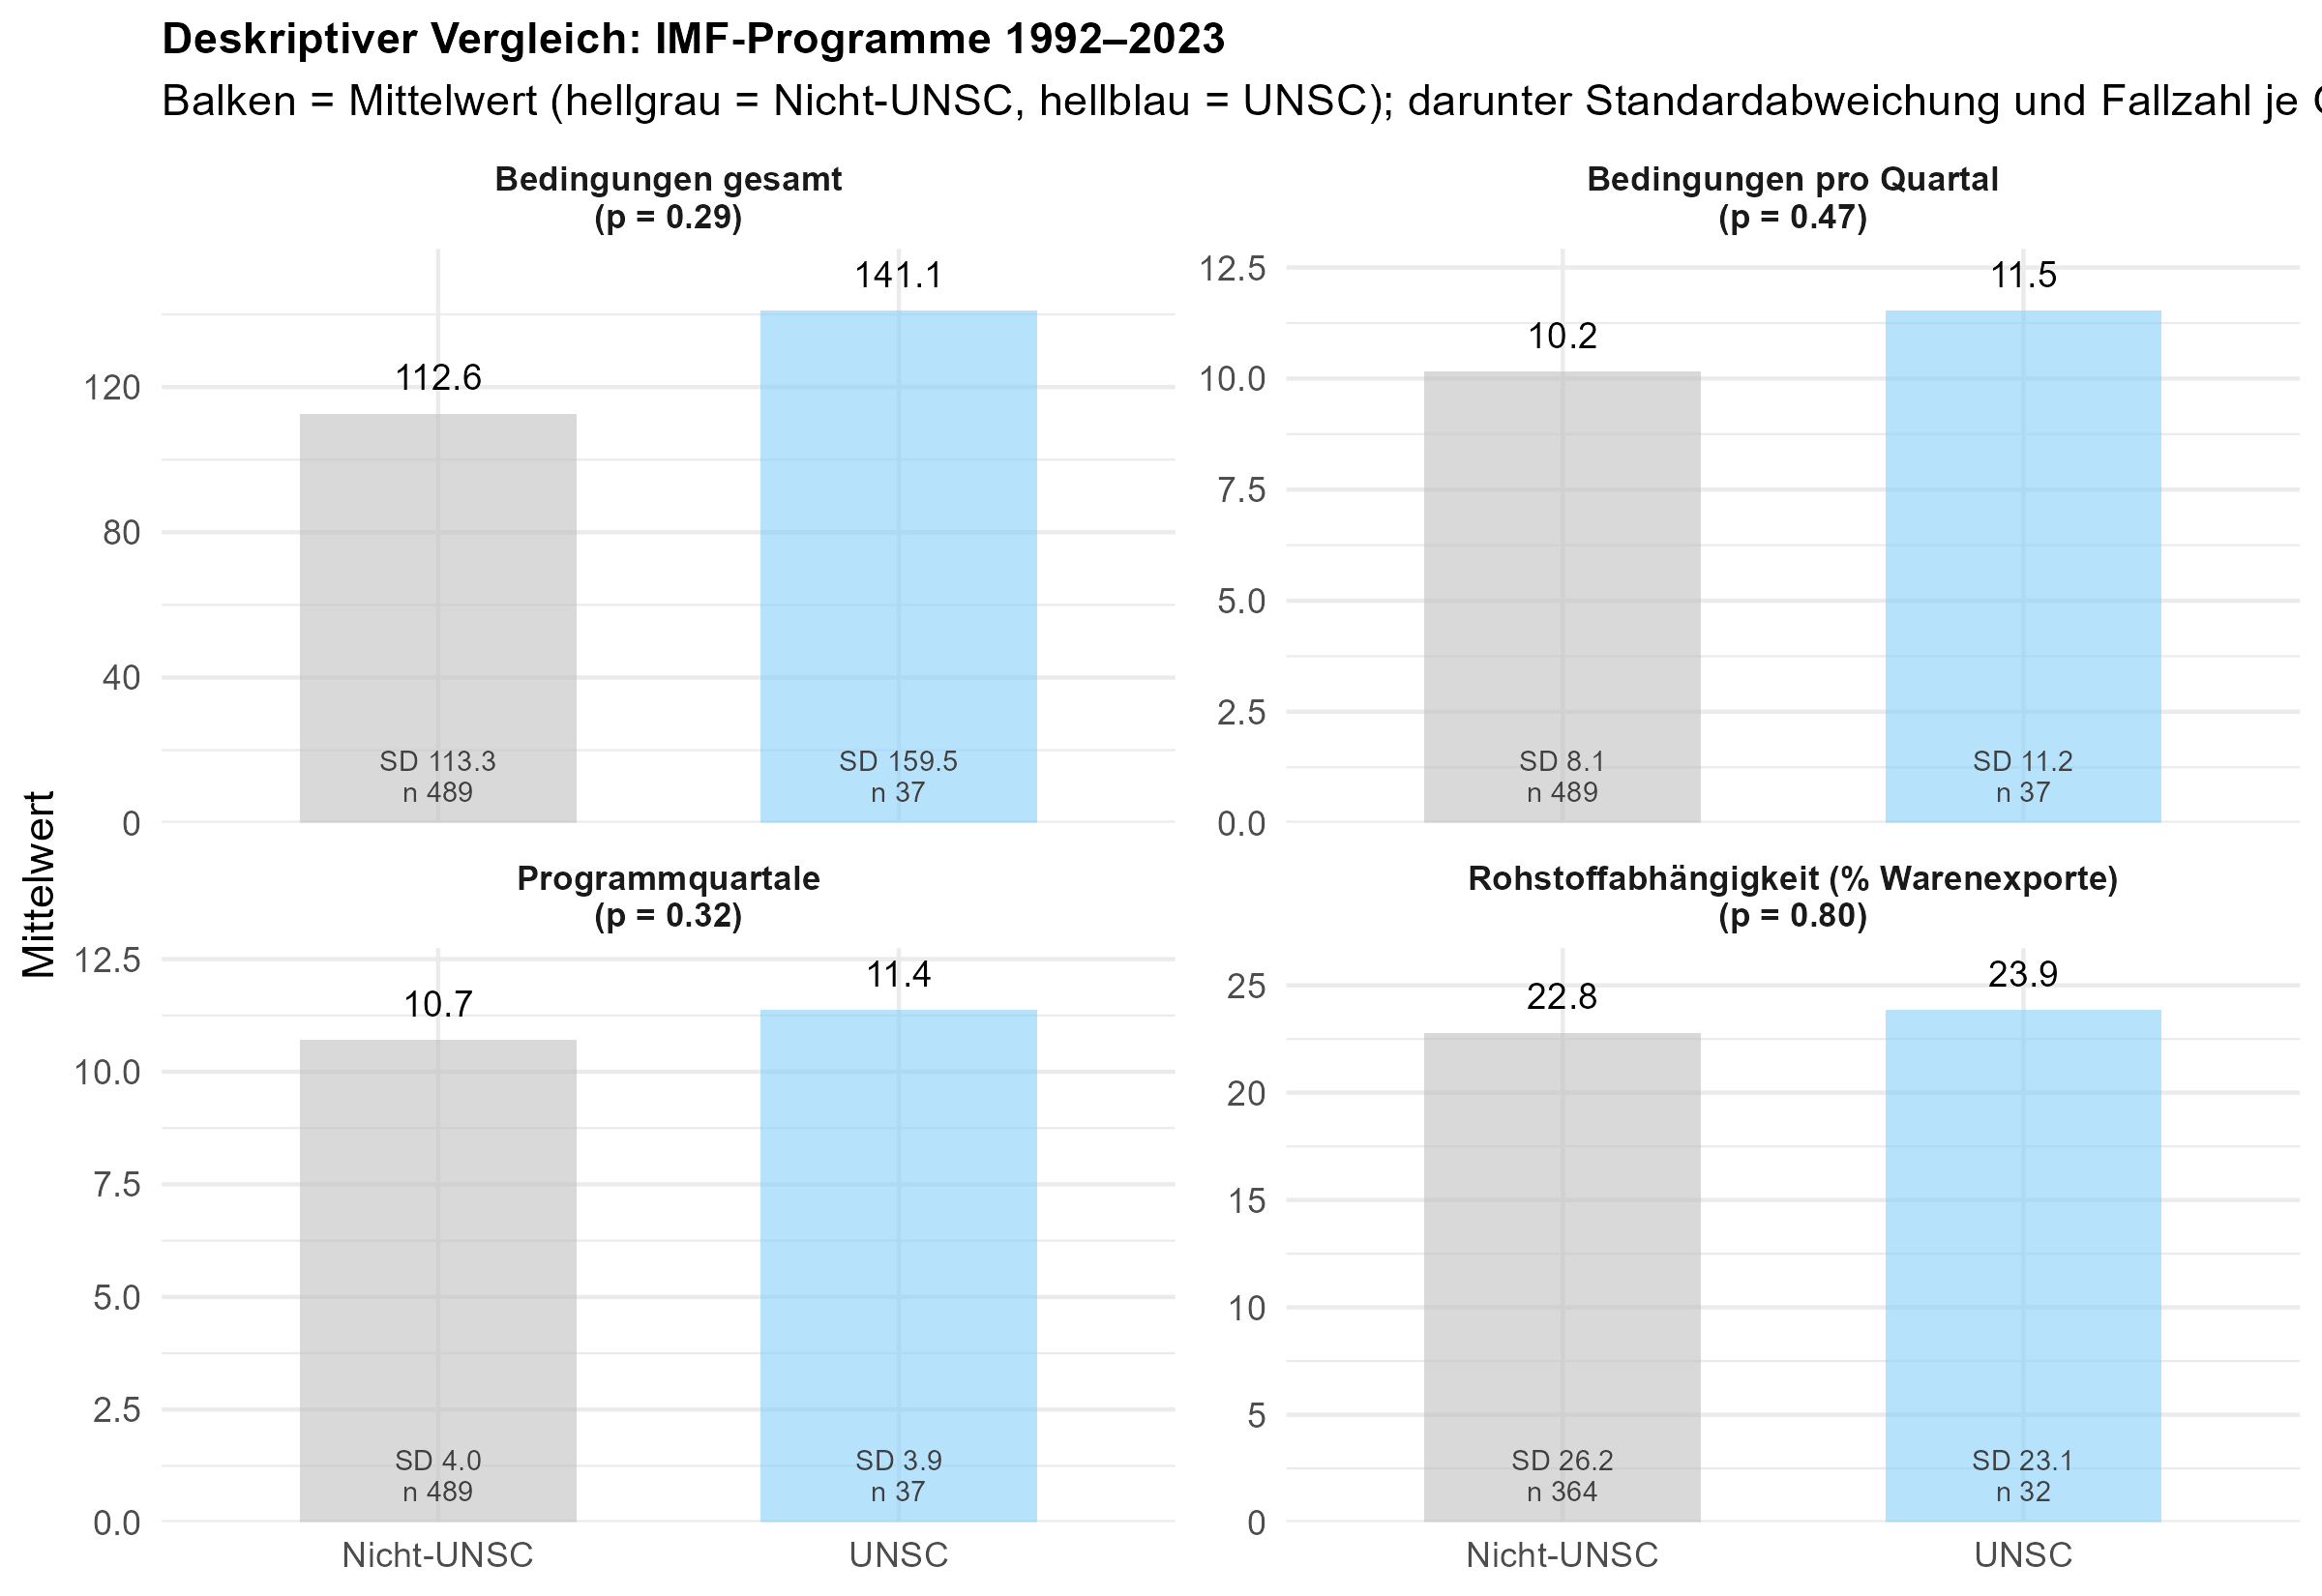
\includegraphics[width=0.85\textwidth]{figures/phase_b/deskriptive_evidenz_gruppe.png}
\caption{Deskriptiver Vergleich UNSC vs.\ Nicht-UNSC, Programm-Land-Jahre 1992--2023 (Balken = Mittelwert; Standardabweichung und Fallzahl je Gruppe unterhalb der Balken; p-Wert des Welch-t-Tests im Paneltitel)}
\end{figure}

Zwei deskriptive Befunde ordnen die Hypothesen ein. Erstens zeigen die \emph{IMF-Programme}, die während einer temporären UNSC-Mitgliedschaft eines Landes bewilligt werden, roh mehr Bedingungen gesamt und eine etwas längere Laufzeit als Programme von Nicht-Mitgliedern; beide Unterschiede sind nicht signifikant. Der Gesamtzähler ist dabei mechanisch laufzeitabhängig: Längere Programme durchlaufen mehr Review-Runden und nehmen mehr Bedingungen auf. Über die Intensität der Konditionalität sagt er deshalb wenig aus; maßgeblich sind die Bedingungen pro Quartal und die Kontrolle der Programmdauer im Modell. Der negativen Erwartung von H1 steht die Rohverteilung damit nicht direkt entgegen, sondern verweist darauf, dass der erwartete Effekt ein Nettoeffekt unter Kontrolle von Programmdauer und Wirtschaftsstruktur ist; wie im Original entsteht der geschätzte Zusammenhang erst in den multivariaten Modellen. Zweitens unterscheiden sich UNSC- und Nicht-UNSC-Jahre in der Rohstoffabhängigkeit praktisch nicht (p um 0{,}8): Die Interaktionsprüfung in H2 wird durch Niveauunterschiede der Rohstoffstruktur nicht vorstrukturiert.

Für H2 wird derselbe deskriptive Vergleich zusätzlich getrennt nach niedriger und hoher Rohstoffexportabhängigkeit (Median-Split, Median 11{,}8 Prozent der Warenexporte) berichtet:

\begin{figure}[h]
\centering
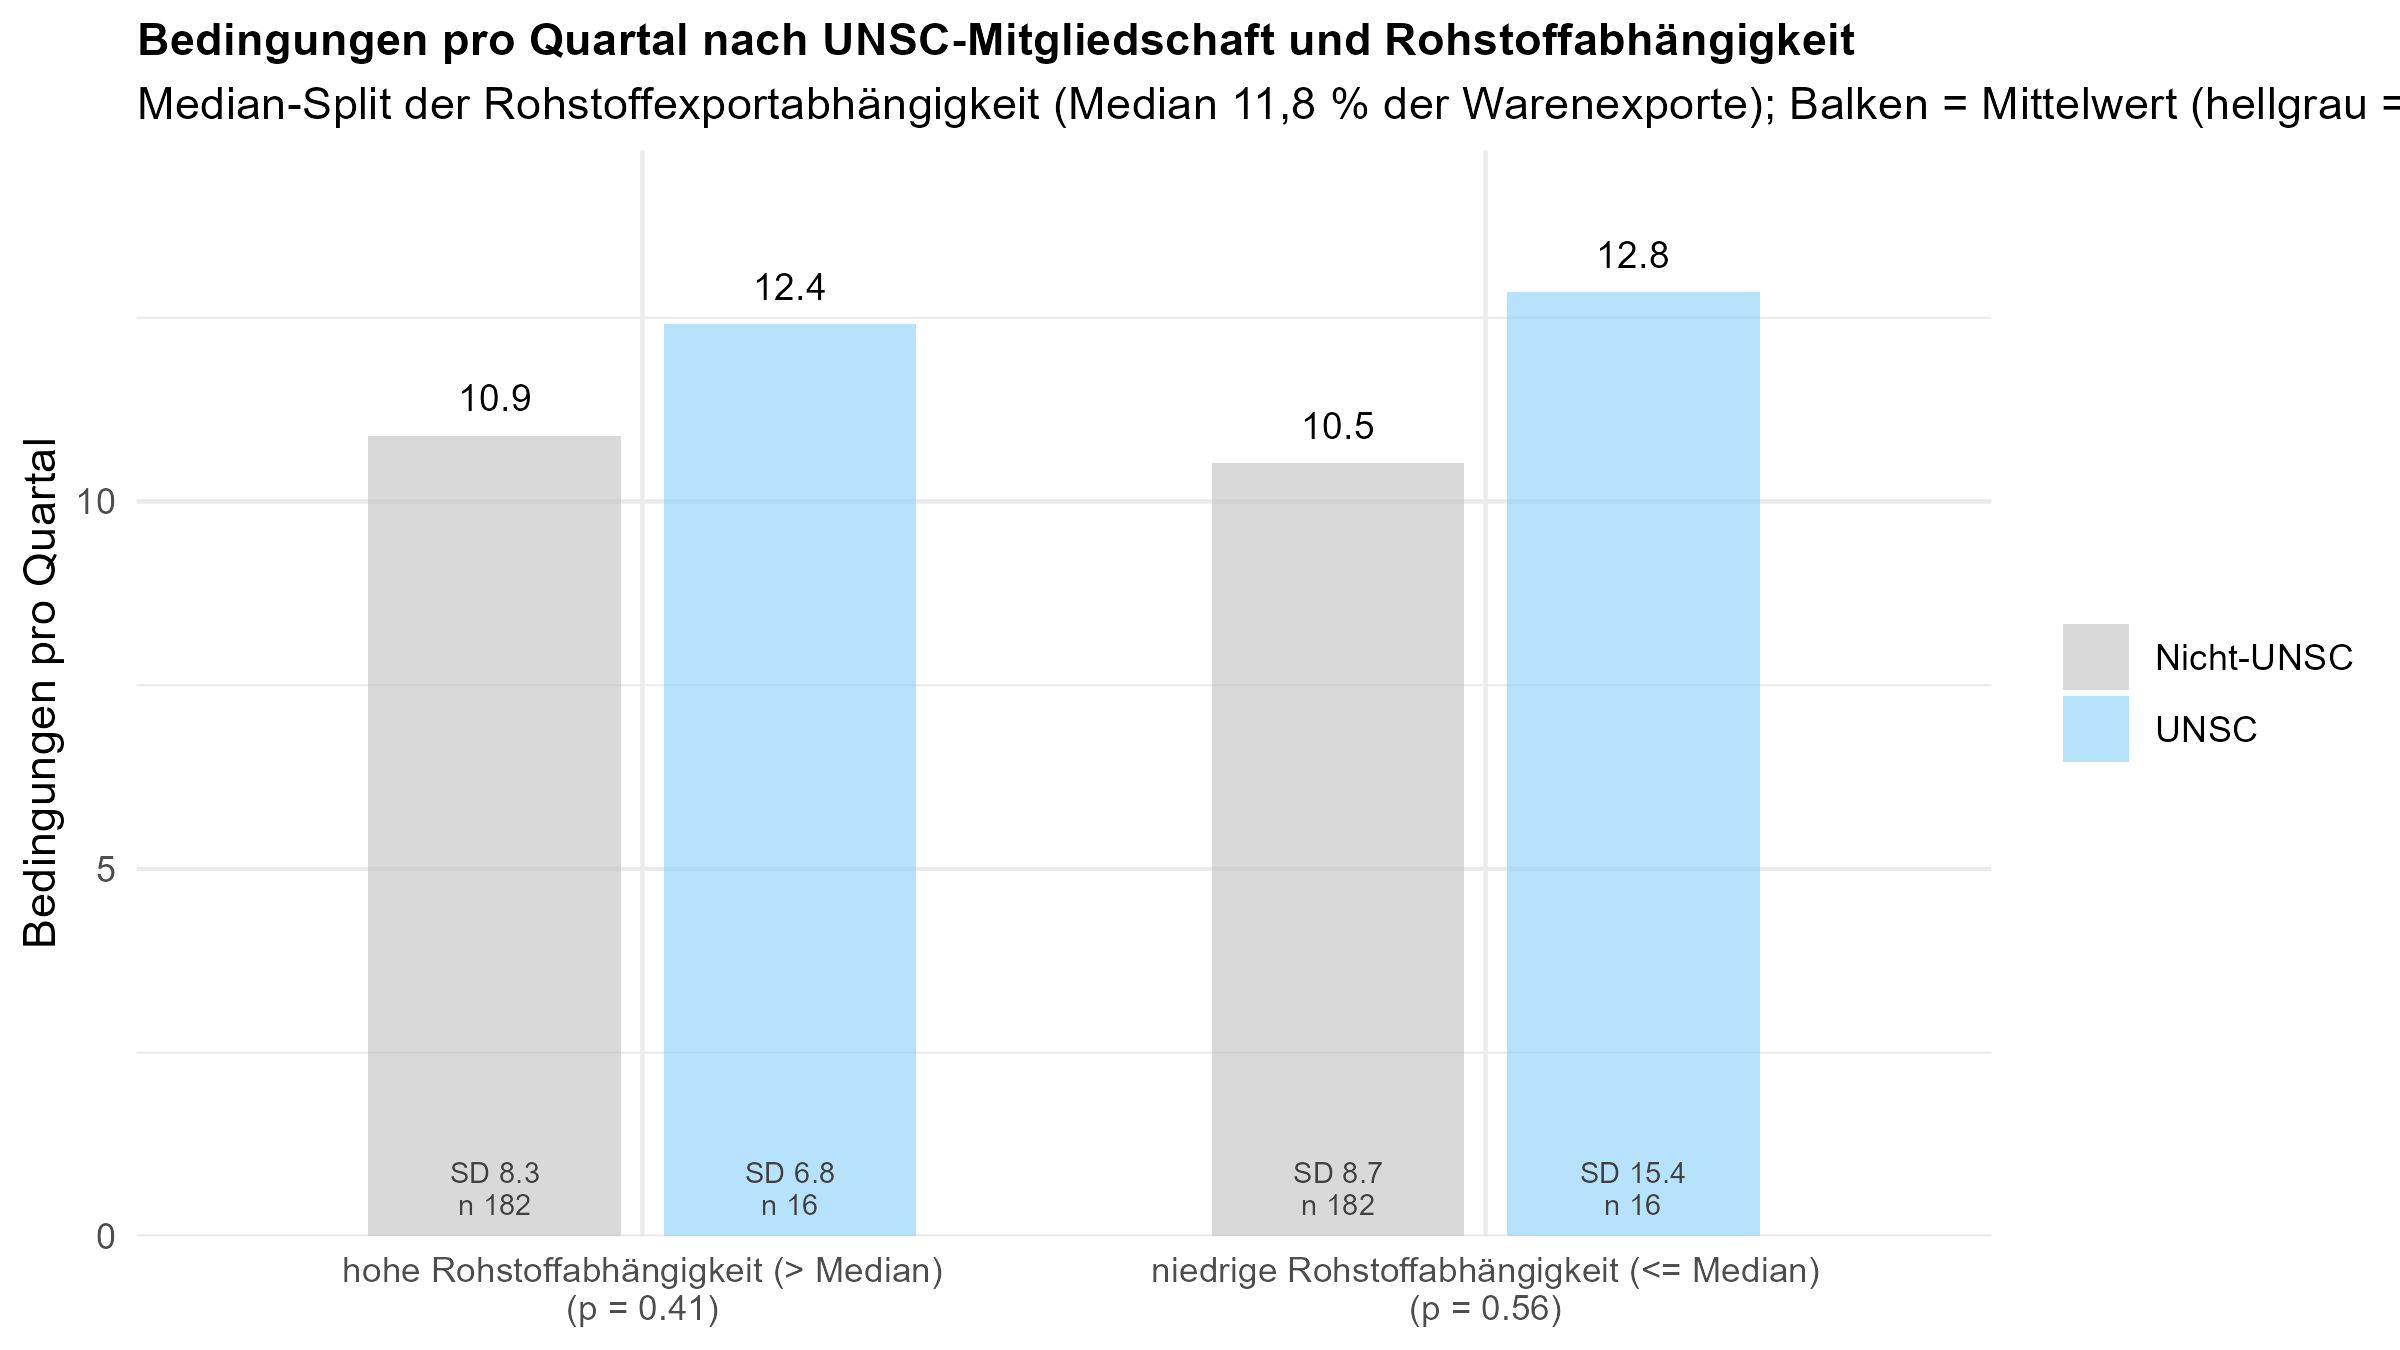
\includegraphics[width=0.85\textwidth]{figures/phase_b/deskriptive_evidenz_h2_split.png}
\caption{Bedingungen pro Quartal nach UNSC-Mitgliedschaft, getrennt nach Rohstoffabh\"angigkeit (Median-Split, Median 11{,}8 Prozent der Warenexporte; Balken = Mittelwert; Standardabweichung und Fallzahl unterhalb der Balken; p-Werte der Welch-t-Tests unter der Achse)}
\end{figure}

Auch hier zeigen sich keine signifikanten Rohunterschiede; die UNSC-Zellen sind klein (je 16 Land-Jahre), sodass die Aufteilung allein der Beschreibung dient.
% Repo-Quelle der Kennzahlen (N je Variable: 489/37 fuer Zaelle und Quartale,
% 364/32 fuer resource_dep, Complete Cases Median-Split: 182/16 je Gruppe):
% code/phase_b/analysis/phase_b_deskriptive_evidenz.R
% results/phase_b/tables/phase_b_deskriptive_evidenz.csv
% results/phase_b/tables/phase_b_deskriptive_evidenz_h2_split.csv



\subsection{Messung und Modellstrategie}
Hier die Operationalisierung, abhängige und unabhängige Variablen sowie Schätzmodell(e) beschreiben.

% TODO vor Abgabe: Formulierung
Die saubere Reihenfolge in der Hausarbeit: H1 und H2 konfirmatorisch testen und als Ihre Ergebnisse berichten → die Quartils-Tabelle im Anhang oder in der Beschreibung der Daten als Kontext („die Programme rohstoffreicher Länder unterscheiden sich inhaltlich“) → und wenn Sie möchten, im Ausblick formulieren: „Für eine künftige Studie böte sich an, die Kompositionshypothese konfirmatorisch zu prüfen, sobald eine belastbarere Klassifikation vorliegt.“ Genau deshalb steht die Bemerkung auch schon so in daten-methodik.tex.

% TODO vor Abgabe: Diese Anmerkung final formulieren oder als
% Robustheits-/Einordnungsabsatz in die Ergebnisse/Diskussion übernehmen.
\paragraph{Anmerkung: Arrangement-Typen und Policy-Areas im Hypothesendesign}
Arrangement-Typen (EFF, PRGF, SBA) und die Verteilung der Bedingungen auf Policy-Areas stehen zwar inhaltlich im Zusammenhang mit Rohstoffabhängigkeit und Stabilisierungsanforderungen. Sie wurden jedoch bewusst nicht als Regressoren oder abhängige Variablen in die konfirmatorischen Hypothesentests (H1, H2) aufgenommen. Dafür gibt es drei Gründe:
\begin{enumerate}
  \item Die klassifikationsbasierte Analyse rohstoff- bzw. stabilitätsbezogener Auflagen entspricht der früheren vierten Hypothese. Sie wurde wegen der unsicheren Operationalisierung aus dem konfirmatorischen Pfad genommen: Die Klassifikation beruht auf einer deterministischen Textregel, und 417 historische MONA-Zeilen ohne Beschreibungstext werden nach der Regel \glqq kein Textsignal = 0\grqq{} als nicht rohstoffbezogen kodiert. Eine Messregel mit dieser Fehleranfälligkeit trägt keinen konfirmatorischen Test und wird ausschließlich explorativ berichtet.
  \item Arrangement-Typen sind potenzielle Mediatoren (post-treatment): Die Fazilität wird zwischen IWF und Land verhandelt. Würde die UNSC-Mitgliedschaft oder die Rohstoffabhängigkeit beeinflussen, welche Fazilität ein Land erhält, würde eine Kontrolle für den Typ den zu schätzenden Gesamteffekt teilweise wegkontrollieren. Auch die Originalstudie nutzt die Arrangement-Typen deshalb nur deskriptiv und zur Stichprobenaufteilung, nicht als Kontrollen im Hauptmodell.
  \item Kompositionsanalysen (welche Policy-Areas von den Bedingungen betroffen sind) wären eigene abhängige Variablen. Für den modernen Zeitraum ab 2009 fehlt eine DSV-identische Messung, weil die Zuordnung moderner MONA-Bedingungen zu den 20 Policy-Areas dieselbe Klassifikationsunsicherheit wie die Rohstoffregel aufweist.
\end{enumerate}
H1 und H2 testen deshalb den Gesamtumfang der Konditionalität (Bedingungen pro Quartal). Die Komposition der Bedingungen wird rein deskriptiv ausgewertet: als Anteil der als rohstoff- bzw. stabilitätsrelevant klassifizierten Bedingungen nach Quartilen der Rohstoffexportabhängigkeit. Ein nachträgliches konfirmatorisches Deuten solcher Kompositionsanalysen würde zudem gegen das Prinzip vorab spezifizierter Hypothesen verstoßen (HARKing); sie sind wie die H3-Länderprofile klar als explorativ zu kennzeichnen.
% Repo-Quelle der deskriptiven Kennzahlen:
% code/phase_b/analysis/phase_b_komposition_exploration.R
% results/phase_b/exploration/komposition_ressourcen_quartile.csv
% results/phase_b/exploration/komposition_ressourcen_quartile_unsc3.csv

\subsection{Abweichungen vom Original und Limitationen}
% ----------------------------------------------------------------------
% SLOT M1 — Abweichungen vom Original (1 Absatz eigene Saetze)
% Muss-Aufzaehlung, alle Punkte im Repo dokumentiert:
% 1. Zeitraum: Phase B 1992-2023 (Panel bis 2025), Original 1992-2008.
% 2. US-Hilfe auf BIP zu Marktpreisen statt Faktorkosten (WDI-Serie endet
%    2008); gemeinsame Jahre 1992-2008: r = 0,98, mediane Abweichung
%    -14 Prozent (steht als TODO bei den Kontrollvariablen).
% 3. Zaehlbasis: ZAehlung ohne Dedup (steht schon in der Datenbasis).
% 4. Handkorrekturen des Originals nicht angewandt (s. SLOT U1).
% 5. H3/H4 nur explorativ: deterministische Textregel; 417 historische
%    MONA-Zeilen ohne Beschreibungstext werden als nicht rohstoffbezogen
%    kodiert (s. Anmerkung-Absatz zu Arrangement-Typen unten).
% 6. AV: Bedingungen pro Quartal statt Gesamtzaehler — der Gesamtzaehler
%    ist laufzeitmechanisch (s. deskriptive Evidenz).
% 7. Zwei-Wege-FE (Laender- UND Jahres-FE) als Hauptspezifikation ist
%    eine bewusste ERGAENZUNG gegenueber DSV (Original-Tabelle 2 ohne
%    Jahres-FE): beggruenden (Epochen-/Krisenjahre absorbieren) und die
%    DSV-nahe GLS-Alternative im Modellvergleich (Anhang) nennen.
% 8. Poisson-FE-Robustheit (H1) folgt Tabelle S2 des Originals
%    (Semi-Elastizitaet, Offset log Quartale).

% SLOT M2 — Limitationen fuer die Auswertung (1 Absatz eigene Saetze)
% Behauptung: kleine UNSC-Zellen beschraenken die statistische Power
% (H2-Vollmodell: 21 unsc3-Jahre in 16 Laendern; Median-Split je 16
% Land-Jahre); Klassifikationsunsicherheit der Rohstoffregel, insbesondere
% post-2008; MONA-Beschreibungstexte historisch uneinheitlich. Deshalb
% Interpretation der Interaktionsmodelle nur vorsichtig-deskriptiv,
% keine kausale Lesart.

\subsection{Robustheitschecks}
Angaben zu Alternative Spezifikationen, Sensitivitätsanalysen oder Heterogenitätschecks.
% NOTIZ (Robustheitsbattery auflisten, s. README-Ergebnistabelle):
% H2: Fuel-/Mineral-Exportvarianten, Placebo Gesamtexporte,
% Winsorisierung (1./99. Perzentil), IMF-Kreditbestand statt
% Nettofluesse; H1: IMF-Kreditbestand, Poisson-FE (S2-Analog),
% Original-Handkorrekturen unsc3 nachgezogen (H1 identisch, H2 in
% 5. Dezimalstelle unveraendert — Kodierungsabweichung ohne Einfluss);
% H2-Zeitfenster 1992-2008 / 2009-2023 (Richtung dreht: +0,274 p=0,012
% bzw. -0,377 p=0,072 — Haupttest bleibt der Gesamtzeitraum);
% Leave-one-country-out (Anhangstabelle).
	


	\section{Ergebnisse}
\label{sec:ergebnisse}

		% Kapitel Ergebnisse der Hausarbeit

\subsection{Hauptbefunde}
Hier die wichtigsten Schätzergebnisse in zusammengefasster Form darstellen.
% SLOT E1 — Hauptbefunde H1 (2-3 eigene Saetze + Verweis auf Anhangstabellen)
% NOTIZ (Zahlen aus results/phase_b/tables/phase_b_modellvergleich.csv und
% phase_b_hypothesen_robustheit.csv — vor Abgabe gegen CSV pruefen):
%   H1 Basismodell (Laender-FE, nur nrquarterssmpl): unsc3 = -0,45 (SE 1,85), p = 0,81, n = 514.
%   H1 Vollmodell (Laender-FE, DSV-Kontrollen): unsc3 = +0,14 (SE 2,82), p = 0,96, n = 282.
%   H1 Hauptmodell (Laender- und Jahres-FE): unsc3 = -0,93 (SE 1,92), p = 0,63, n = 281, davon 24 unsc3-Jahre.
% Fazit H1: kein signifikanter Effekt im modernen Zeitraum (1992-2023),
% anders als im Originalzeitraum (dort ca. 30 Prozent weniger Konditionen).

% SLOT E2 — Hauptbefunde H2/H4 (2-3 eigene Saetze)
% NOTIZ (Zahlen aus phase_b_hypothesen_robustheit.csv,
% phase_b_h2_leave_one_country_out.csv, phase_b_h4_leave_one_country_out.csv):
%   H2 Hauptmodell: unsc3:resource_dep = -0,11 (SE 0,10), p = 0,29, n = 212.
%   H2 Robustheit Fuel-Exporte: -0,22, p = 0,024 — EINZIGE signifikante Spezifikation.
%   H2 Robustheit Mineral-Exporte: +0,01, p = 0,91. Placebo (ExportGDP): -0,12, p = 0,37.
%   H4 explorativ (s. Tab. 7, phase_b_h4_ergebnisse.tex): Interaktion -1,93e-06 (SE 4,96e-04), p = 0,997, n = 212; Robustheiten Fuel/Mineral/Kreditbestand/winsor alle n.s.; Zeitfenster 1992-2008 p = 0,307, 2009-2023 p = 0,706.
%   Leave-one-out (H2): ohne PER -0,19, ohne GAB -0,04 → die Interaktion
%   haengt an einzelnen Laendern (Instabilitaet erwaehnen).
%   H2-Zeitfenster: 1992-2008 +0,27 (p = 0,012, signifikant POSITIV),
%   2009-2023 -0,38 (p = 0,072) — die Interaktionsrichtung DREHT
%   zwischen den Fenstern; in der H2-Interpretation sauber einordnen
%   (Haupttest: Gesamtzeitraum; Fenster sind Robustheit).
%   H1 Poisson-FE (S2-Analog): -0,043, p = 0,78 — Semi-Elastizitaet
%   ca. 4 Prozent weniger Bedingungen pro Quartal, nicht signifikant.
% ACHTUNG: Der bestehende Satz "kein stabiler signifikanter Effekt" im
% Interpretation-Absatz unten muss die Fuel-Export-Ausnahme (p = 0,024)
% und die Leave-one-out-Sensitivitaet sauber einordnen.


\subsection{Interpretation}
Interpretation der Richtung, Stärke und Bedeutung der Effekte in der Sprache der Forschung.
% SLOT E3 — Sprechweise: Punktschaetzer vs. Unsicherheit (kein eigener
% Absatz noetig; die Unterscheidung nur in den Interpretations-Saetzen
% anwenden, danach diesen Marker entfernen)
% NOTIZ (Begriffsklaerung als Schreibhilfe — NICHT als Lehrbuch-Definition
% in die Arbeit uebernehmen):
% - Punktschaetzer = der einzelne Zahlenwert des Koeffizienten, der
%   "Rat" des Modells: z.B. H2-Interaktion -0,11.
% - Standardfehler = typische Unsicherheit des Rats (hier 0,10).
% - p-Wert = Wahrscheinlichkeit, mindestens ein so grosses
%   Punktschaetzer-Ergebnis zu sehen, wenn der wahre Wert null waere
%   (hier 0,29).
% Formulierungsregeln fuer die eigenen Saetze:
% - "Der Punktschaetzer zeigt Richtung X" ist KEIN Beweis fuer X.
% - Insignifikant heisst "nicht von null unterscheidbar", NICHT
%   "belegt null" (vgl. Zeitfenster 2002-2008: -1,86 bei p = 0,52).
% - Musteranwendung Differenztest: "Die Punktschaetzer sprechen fuer
%   eine Abschwaechung des Effekts nach 2002 (+2,5), der formale Test
%   verfehlt jedoch die Signifikanz (p = 0,36)."


In den Robustness-Checks zeigt sich kein stabiler signifikanter Effekt von UNSC-Mitgliedschaft, Ressourcenabhängigkeit 
oder ihrer Interaktion auf die IMF-Konditionalität. 
Die Ergebnisse sind insgesamt inkonsistent und sprechen eher gegen einen robusten Moderationseffekt.

Das heißt: Die Daten liefern in diesem Spezifikationsrahmen keine belastbare Evidenz für einen signifikanten Haupteffekt 
oder einen signifikanten gemeinsamen Effekt.
% ----------------------------------------------------------------------
% INTERPRETATION H1-H3 — eigener Entwurf (2026-10-05), faktisch
% korrigiert. Verbleibende Pruefpunkte als TODO am jeweiligen Block.
% ----------------------------------------------------------------------
Die Zerlegung des Originalzeitraums zeigt, dass der publizierte Effekt zeitlich von den 1990er-Jahren getragen wird: In den Punktschätzern zeichnet sich bereits Anfang und Mitte der 2000er, begleitet vom Rückgang der Nachfrage nach IMF-Krediten \parencite[545]{KentikelenisIMFConditionalityDevelopment2016}, eine Abschwächung ab; der formale Differenztest verfehlt allerdings wegen der kleinen Stichprobe die Signifikanz. Mit dem über den Originalzeitraum hinaus bis 2023 erweiterten Panel lässt sich dieser Trend weiter beobachten. Der Nullbefund ist dabei kein Artefakt der IMF-Inaktivität: Auch in der Phase massiver Nachkrisen-Kreditvergabe ab 2009 zeigt sich kein UNSC-Effekt. Als Deutungsangebot bietet sich an, dass die Einflusskauf-Logik an die geopolitische Konstellation der 1990er gebunden war und nach deren Ende an Bedeutung verlor.
% TODO (H1): Zeitfenster-Tabelle (original_replication_zeitfenster) fehlt
% bisher im Anhang — entweder aufnehmen oder die Zerlegung hier nur
% verbal belegen (1992-2001: -4,65; 2002-2008: -1,86).
% TODO (H1): Momani & Helleiner 2007 nicht in literatur.bib — als
% Sekundaerzitat ueber Kentikelenis et al. belassen oder nachtragen.

Die Behauptung, die Rohstoffabhängigkeit moderiere den UNSC-Effekt derart, dass sich dieser in rohstoffabhängigeren Ländern stärker zugunsten der UNSC-Mitglieder — in noch weniger Bedingungen — ausprägt, lässt sich nicht bestätigen. Nur in einer Spezifikation, die Rohstoffabhängigkeit ausschließlich über die Erdöl-Exportquote misst, zeigt sich eine signifikante Moderation; die Mineral- und Placebo-Varianten bleiben null, und die Leave-one-out-Analyse zeigt, dass die Hauptinteraktion von einzelnen Ländern abhängt. Ein Allgemeineffekt lässt sich von der Erdöl-Spezifikation nicht ableiten.
% TODO (H2): Tabellenverweise ergaenzen (Anhang: H2-Ergebnisse,
% H2-Modellvergleich, Robustheitstabelle) und gegen das PDF pruefen.

Die Länder im untersten Quartil der Konditionalität (2,0 bis 7,2 Bedingungen pro Quartal) sind in Bezug auf die Rohstoffabhängigkeit heterogen verteilt: von Äthiopien (0,8\,\%) und Mali (0,6\,\%) über Kenia (12,7\,\%) bis Peru (43,6\,\%); selbst der Irak (98,6\,\%) liegt mit 7,8 Bedingungen nur marginal über der Quartilsgrenze. Unter den Ländern mit den höchsten Konditionalitäten (75. Perzentil bis Maximum, 12,5 bis 40,5 Bedingungen) reicht die Spanne von Irland (31,4 Bedingungen bei 2,3\,\% Rohstoffabhängigkeit) über Griechenland (17,7 bei 40,4\,\%) bis Angola (20,3 bei 99,3\,\%); Portugal markiert mit 40,5 Bedingungen bei 10,4\,\% das Maximum. Aus der Rohstoffabhängigkeit allein lassen sich daher keine systematischen Zusammenhänge mit der Höhe der Bedingungen pro Quartal ableiten. Im Innerhalb-Länder-Vergleich der UNSC-Länder (die vollständigen Länderprofile sind als Reproduktionsmaterial im Repository der Arbeit einsehbar) zeigt sich dieselbe Heterogenität anhand der Differenzen zwischen den Bedingungs-Mittelwerten in UNSC-Jahren und Nicht-UNSC-Jahren: Unter den rohstoffabhängigeren UNSC-Ländern mischen sich positive Lücken (Niger +14,7, Ruanda +16,4, Ägypten +7,2, Mosambik +3,4) und negative (Gabun -4,3, Guinea -9,9). Die Lückenfolge folgt somit nicht der Rohstoffabhängigkeit — konsistent mit dem H2-Nullbefund.
% TODO (H3): Die Quartils-/Perzentilwerte stammen aus den
% Explorationstabellen (konditionalitaet_perzentile etc.), die nicht
% Teil der Hausarbeit sind — fuer die Abgabe entweder als eigene
% Berechnung im Anhang dokumentieren oder die Formulierung vollstaendig
% auf Tabelle 6 stuetzen.



\begin{figure}[h]
\centering
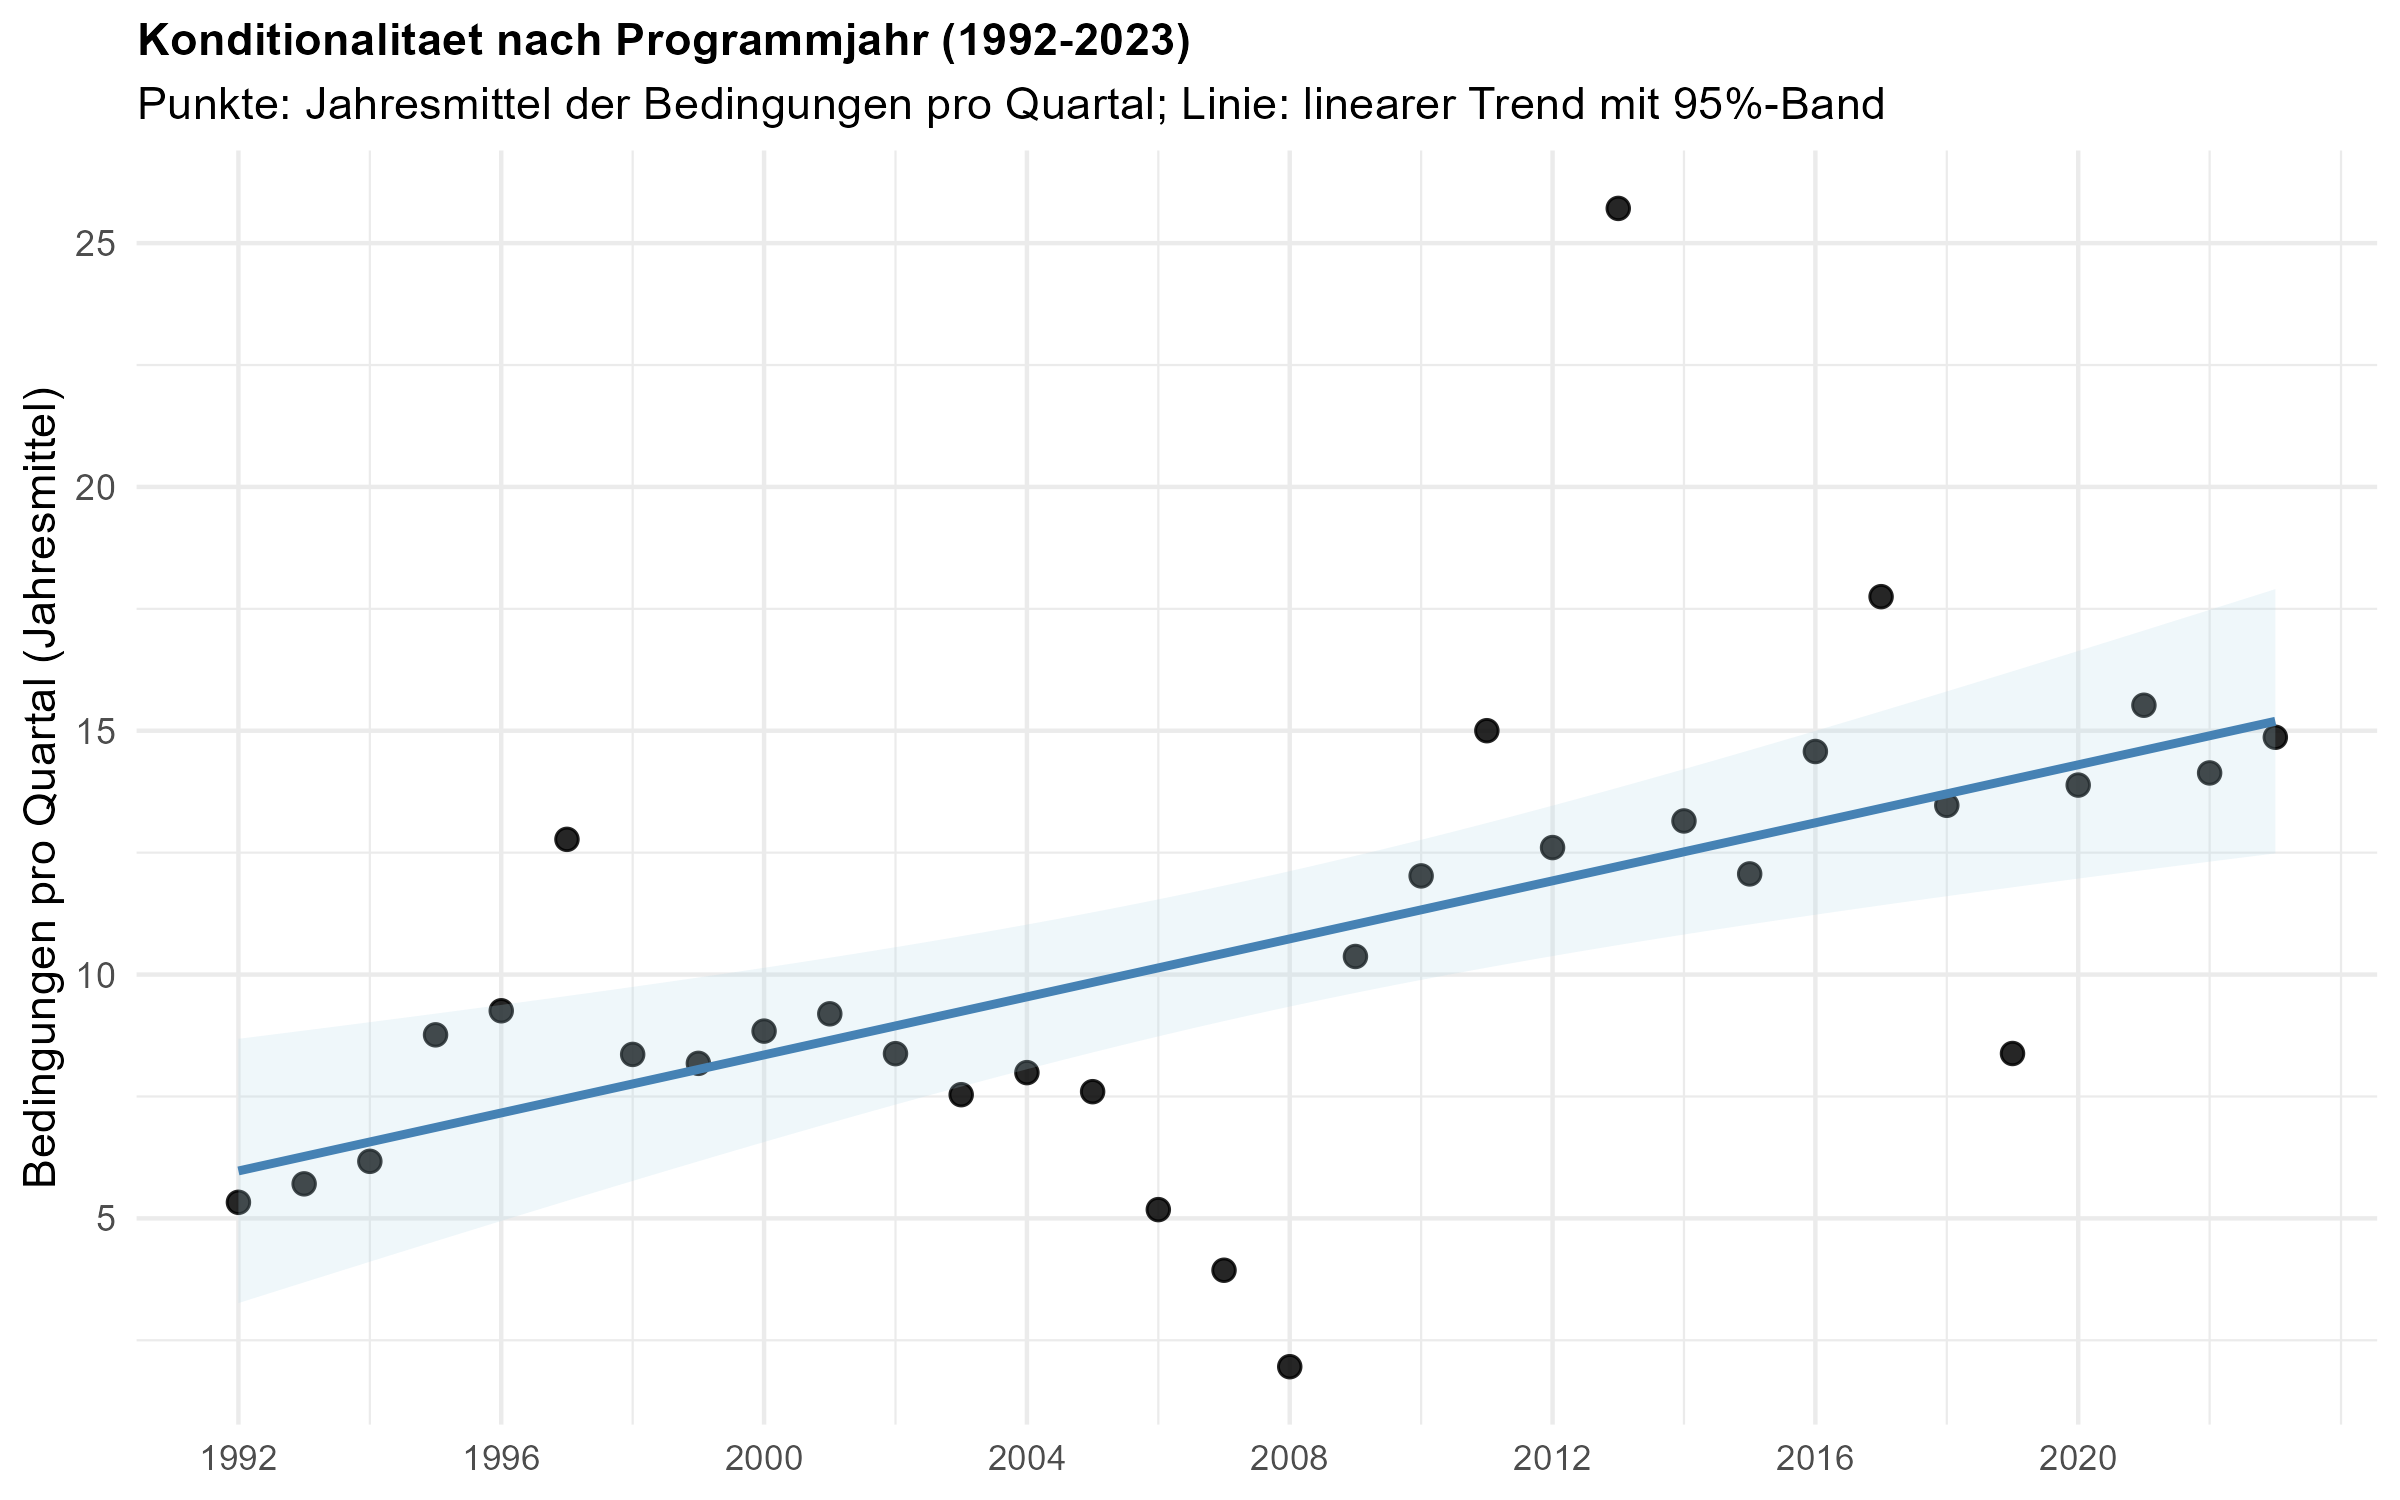
\includegraphics[width=0.85\textwidth]{figures/phase_b/konditionalitaet_jahresreihe.png}
\caption{Bedingungen pro Quartal nach Programmjahr, 1992--2023 (Punkte: Jahresmittel; Linie: linearer Trend mit 95-Prozent-Band). Deskriptive Kontextdarstellung; die Jahres-Fixed-Effects der Modelle absorbieren dieses Niveau.}
\label{fig:konditionalitaet-jahresreihe}
\end{figure}

% SLOT E4 — Verweis-Satz auf die Abbildung (1-2 eigene Saetze)
% Behauptung: Die Abbildung zeigt den Epochenwechsel: historisches
% Nachfragetief 2008 (nur 6 Programmjahre, 2,0 Bedingungen/Quartal),
% danach Anstieg auf rund das Doppelte des 1990er-Niveaus (Spitze 2013).
% Verknuepfen mit der H1-Einordnung (SLOT E1) und dem IMF-Rueckkehr-
% Argument (SLOT D1 in diskussion.tex, Kentikelenis et al. S. 545).
% Daten: results/phase_b/exploration/konditionalitaet_jahresreihe.csv;
% Skript: code/phase_b/analysis/phase_b_ressourcen_exploration.R,
% Sektionen F (Daten) und G (Abbildung).

% TODO vor Abgabe: Diese Anmerkung final formulieren oder als
% Robustheits-/Einordnungsabsatz in die Ergebnisse/Diskussion übernehmen.
\paragraph{Explorative Zusatzanalyse: Komposition der Bedingungen}
Die Komposition der Bedingungen wird rein deskriptiv ausgewertet (Skript
\texttt{code/phase\_b/analysis/phase\_b\_komposition\_exploration.R}; Output
\texttt{results/phase\_b/exploration/komposition\_ressourcen\_quartile.csv}
sowie \texttt{.../komposition\_ressourcen\_quartile\_unsc3.csv}). Stichprobe:
396 Land-Jahre mit \texttt{resource\_dep} (1992--2023); Quartilsgrenzen der
Rohstoffabhängigkeit bei 3{,}8 / 11{,}8 / 35{,}3 Prozent der Warenexporte.

\begin{table}[h]
\centering
\begin{tabular}{lrrr}
\hline
Quartil & Bedingungen & Rohstoff-Anteil (gew.) & Stabilitäts-Anteil \\
\hline
Q4 (hoch) & 12.471 & 3{,}7 \% & 28{,}9 \% \\
Q3 & 12.297 & 4{,}1 \% & 29{,}4 \% \\
Q2 & 12.722 & 2{,}3 \% & 26{,}6 \% \\
Q1 (niedrig) & 10.858 & 2{,}3 \% & 26{,}0 \% \\
\hline
\end{tabular}
\caption{Anteil rohstoff- bzw. stabilitätsklassifizierter Bedingungen nach Quartilen der Rohstoffexportabhängigkeit (deskriptiv, gewichtete Anteile)}
\end{table}

Deskriptiv zeigt sich der erwartbare Gradient: In der oberen Hälfte der
Rohstoffabhängigkeit liegt der Anteil explizit extraktivbezogener Bedingungen
fast doppelt so hoch wie unten (4{,}1 bzw. 3{,}7 Prozent gegen 2{,}3 Prozent),
während der Stabilitätsanteil weitgehend flach bleibt. Im Quartil-$\times$-UNSC-Schnitt
(sehr kleine UNSC-Zellen, 6--10 Fälle je Quartil) liegt der Rohstoffanteil bei
UNSC-Jahren durchweg niedriger als bei Nicht-UNSC-Jahren — ein Zahlenmuster,
das zur H2-Richtung passt, aber wegen Zellgröße und Klassifikationsunsicherheit
nur als Beschreibung taugt. Die Einschränkungen (417 historische Zeilen ohne
Beschreibungstext werden als nicht rohstoffbezogen kodiert; keine Inferenz)
dokumentiert das Skript mit.

% ----------------------------------------------------------------------
% INTERPRETATION H4 — eigener Entwurf (2026-10-05), faktisch korrigiert.
% ----------------------------------------------------------------------
H4 wurde aufgrund der Klassifikationsunsicherheit der selbst definierten Rohstoff- und Stabilitätsklassifikationen aus dem konfirmatorischen Pfad genommen; die Analyse der Bedingungsinhalte in Kombination mit der UNSC-Mitgliedschaft ist als rein explorativ zu verstehen. Die explorative Schätzung ergibt keine Moderation durch die UNSC-Mitgliedschaft: Die Veränderung über die gesamte Spannweite der Rohstoffabhängigkeit beträgt weniger als 0{,}02 Prozentpunkte, und in keiner Spezifikation zeigt sich ein Muster, das die Kompositionshypothese stützen würde. Abwegig ist der Rohstoff-Ansatz allerdings nicht: Über die Quartilstabelle (Tabelle 1) lässt sich zumindest deskriptiv eine plausible Korrelation der Klassifikation mit der Rohstoffabhängigkeit ablesen — ein Hinweis auf inhaltliche Validität. In der oberen Hälfte der Rohstoffabhängigkeit liegt der Anteil rohstoffbezogener Bedingungen deutlich höher als in der unteren, wobei der Gradient aus zwei Gründen leicht ausfällt: Der Absolutwert liegt selbst in Q3/Q4 nur bei 4{,}1 bzw. 3{,}7 Prozent, und der Anstieg verläuft nicht monoton, sondern verdoppelt sich nur im Übergang von der unteren zur oberen Hälfte. Relativ zum Niveau betrachtet ist das Muster dennoch spezifisch: Der Stabilitätsanteil schwankt um weniger als ein Zehntel seines Niveaus (26{,}0 bis 28{,}9 Prozent), während sich der Rohstoffanteil verdoppelt — die Verschiebung betrifft also gezielt den Rohstoff-Inhalt und ist keine bereichsübergreifende Dynamik. Kritisch ist anzumerken, dass der Gradient teilweise mechanisch sein kann, da Bedingungen mit Rohstoffbezug nur dort auftreten, wo ein Rohstoffsektor ökonomisch bedeutsam ist. Insgesamt bleibt die Kompositionshypothese damit ein Kandidat für eine Folgestudie mit belastbarerer Klassifikation.
% TODO (H4): Tabellenverweise (Tabelle 1, Tabelle 7) gegen das
% kompilierte PDF pruefen; ggf. \cref statt fester Nummern verwenden.


\section{Diskussion}
\label{sec:diskussion}

		% Kapitel Diskussion der Hausarbeit
% ----------------------------------------------------------------------
% GERUEST-Konventionen: wie sections/theorie.tex (SLOT/NOTIZ/TODO).
% Vor Abgabe muessen alle SLOT/NOTIZ/TODO-Marker aufgeloest sein.

% SLOT D1 — Einordnung der Befunde (2-3 eigene Saetze)
% Behauptung: den H1-Nullbefund im modernen Zeitraum (1992-2023) vor dem
% Hintergrund des Originals einordnen (dort ca. 30 Prozent weniger
% Konditionen). Moegliche Erklaerungen, abwaegen: veraenderte
% Konditionalitaetspraxis nach 2008, zu kleine UNSC-Zellen (Power-Problem),
% oder tatsaechlich nachlassende Geberlogik der Hauptanteilseigner.
% WICHTIG: die Fuel-Export-Ausnahme (p = 0,024) nicht ueberbewerten —
% eine einzige Spezifikation von vielen (Mineral-Variante p = 0,91,
% Placebo gesamte Exporte p = 0,37). Leave-one-out existiert NUR fuer
% die HAUPTinteraktion resource_dep (dort: Abhaengigkeit von PER/GAB);
% fuer die Fuel-Spezifikation selbst liegt kein LOO-Befund vor.
% NOTIZ (eigenes Phase-A-Ergebnis — staerkstes Argument hier):
% Auf den ORIGINALDATEN gilt (s. docs/session_protokoll_2026-09-24.md
% und Ergebnistabelle original_replication_zeitfenster; Zahlen vor
% Abgabe gegen die Tabelle pruefen):
%   1992-2001: unsc3 = -4,65 (p = 0,042) — Effekt signifikant.
%   2002-2008: unsc3 = -1,86 (p = 0,52) — statistisch Null.
% D.h. der publizierte Effekt wird von den 1990ern getragen und ist
% ab 2002 selbst auf Originaldaten null. Der Phase-B-Nullbefund
% (1992-2023) ist damit KEIN Replikationsfehler, sondern bildet einen
% realen zeitlichen Rueckgang ab. Achtung fuer die Formulierung: Das
% Originalpapier selbst berichtet KEINE Subperioden-Zerlegung — die
% Einsicht stammt aus der eigenen Phase-A-Analyse und muss so
% (als eigener Befund) zitiert werden, nicht DSV zugeschrieben werden.
% ERGAENZUNG (direkter Differenztest, phase0_replikation_original.R):
% Interaktion unsc3 x ab2002 — Basis: +2,54 (SE 2,74, p = 0,36);
% Vollmodell: +5,21 (SE 5,42, p = 0,34); Tabelle
% results/phase_a/tables/original_replication_zeitfenster_interaktion.csv.
% Richtung wie erwartet (Effekt nach 2002 deutlich schwächer Richtung
% Null), aber die Differenz ist auf dem kleinen Sample NICHT
% signifikant. In der Arbeit ehrlich beides berichten: signifikante
% Fruehperiode + Null spät + nicht-signifikanter Differenztest.
% NOTIZ (Finanzkrise/IMF-Rueckkehr, verifiziert gegen Kentikelenis et al.
% 2016 — alle drei Stellen auf ARTIKEL-S. 545, Tab.-1-Diskussion ca. S. 551):
% - Mitte der 2000er: Nachfrage nach IMF-Krediten auf historischem Tief,
%   Zweifel an der Zukunft des IMF (dort zitieren die Autoren Momani und
%   Helleiner 2007 — Original NICHT in literatur.bib: entweder Bib-Eintrag
%   + eigene Lektuere nachtragen ODER als Sekundaerzitat nur ueber
%   Kentikelenis et al. laufen lassen).
% - 2009: G-20-Zusagen von 750 Mrd. USD; 2009-2014 insgesamt 129 neue
%   Kredite an 76 Laender (Artikel-S. 545).
% - Post-2008: Konditionen-Median sinkt kurzfristig (von ca. 42 in
%   1996-2007 auf 33-35), steigt bis 2014 wieder auf 44; Zahl aktiver
%   Programme nimmt nach der Krisenspitze wieder ab.
% Verwendung im Argument: Der Phase-B-Nullbefund ist KEIN Artefakt der
% IMF-Inaktivitaet — auch in der Phase massiver Nachkrisen-Kreditvergabe
% zeigt sich kein UNSC-Effekt im erweiterten Panel. Caveat: Nachkrisen-
% programme unterscheiden sich in Typ und Zusammensetzung von den
% BOP-Krisen der 1990er; die Einflusskauf-Logik war an deren geopolitische
% Konstellation geknuepft (vgl. Originalpapier: Zimbabwe/Irak 1992).
% Quellen: \parencite[TODO]{DreherPoliticsIMFConditionality2015},
% \parencite[TODO]{KentikelenisIMFConditionalityDevelopment2016},
% \parencite[TODO]{StubbsHowEvaluateEffects2020} (Endogenitaet,
% Identifikation, Evaluationsproblematik).

% SLOT D2 — Limitationen buendeln (2 eigene Saetze)
% Behauptung: die Daten-/Klassifikationslimitationen (SLOT M1/M2 in
% daten-methodik.tex) hier als Methodik-Diskussion zusammenfuehren, nicht
% als reine Fehlerliste: was koennen die Modelle deshalb aussagen und was
% nicht (deskriptiv-vorsichtig, keine kausale Lesart).

% SLOT D3 — Abhaengigkeitstheoretische Lesart (1-2 eigene Saetze)
% Behauptung: aus der Rahmung in theorie.tex (SLOT 4/5) folgt: ein
% ausbleibendes "Entgegenkommen" fuer rohstoffreiche Laender (H2-Null,
% H4-Null) spricht gegen eine Machtressourcen-Logik im modernen
% Konditionalitaetsregime — oder dafuer, dass deren Mechanismus nach 2008
% an Bedeutung verloren hat. Formulierung braucht Sorgfalt, weil H2/H4
% nur explorativ getestet wurden.
% Quellen: \parencite[TODO]{MuchhalaExaminingFeaturesEconomic2025},
% \parencite[TODO]{AntunesDeOliveiraDependencyTheory2024}.
% NOTIZ (fakultativ, 1 Satz): Auch auf der Outcome-Seite kein Muster —
% Konditionalitaetsintensitaet korreliert nicht mit der Veraenderung
% der Rohstoffexportabhaengigkeit t bis t+3 (Spearman rho = 0,039,
% n = 333 Programm-Landjahre; h4_conditionality_resource_change_3y):
% kein Beleg dafuer, dass Konditionalitaet Rohstofforientierung
% systematisch auf- oder abbaut — in keine Richtung.

\subsection{Beitrag der Arbeit}
% SLOT D4 — Beitrag (2-3 eigene Saetze)
% Behauptung: die Replikation uetraegt das DSV-Design auf den modernen
% Zeitraum 1992-2023 und zeigt: der Originalbefund laesst sich nicht
% ohne weiteres fortsetzen. Explorative H3/H4-Ergebnisse liefern
% Hypothesen fuer Folgestudien (Kompositionshypothese konfirmatorisch
% pruefen, sobald eine belastbarere Policy-Area-Klassifikation vorliegt).

% SLOT D5 — Ausblick (1-2 eigene Saetze, optional)
% Behauptung: konfirmatorische Erweiterungen nennen: eigene
% Policy-Area-Klassifikation fuer post-2008-Bedingungen, groessere
% Zahl UNSC-Fenster im Panel, alternativ IMF-Kreditbestand statt
% Nettofluesse (bereits gerechnet, s. Robustheitstabelle).


	\section{Fazit}
% NOTIZ (Fazit-Checkliste — vor Abgabe aufloesen):
% 1. Kernbefunde H1/H2 in 2-3 Saetzen zusammenfassen — KEINE neuen
%    Zahlen, keine neuen Argumente; das Fazit fasst nur zusammen.
% 2. Zeitliche Einordnung als roten Faden nennen: Effekt der 1990er,
%    kein Artefakt der IMF-Inaktivitaet (Nachkrisen-Kreditvergabe).
% 3. Beitrag der Arbeit: Replikation mit Zeiterweiterung; explizite
%    Explorationsstruktur H3/H4 als methodische Sauberkeit.
% 4. Limitationen in 1-2 Saetzen (kleine UNSC-Zellen,
%    Klassifikationsunsicherheit, Datenluecken bei resource_dep).
% 5. Ausblick: konfirmatorische Kompositionshypothese mit
%    belastbarerer Klassifikation; ggf. Zeitfenster-Projektion.
	
	
	\section{Appendix}
	\onehalfspacing
	% LaTeX table fragment. Requires \usepackage[utf8]{inputenc}, \usepackage{booktabs,longtable,array}, and \usepackage{pdflscape}.
\begingroup
\scriptsize
\setlength{\tabcolsep}{3pt}
\begin{landscape}
\begin{longtable}{>{\raggedright\arraybackslash}p{3.5cm}>{\raggedleft\arraybackslash}p{1.54cm}>{\raggedleft\arraybackslash}p{1.54cm}>{\raggedleft\arraybackslash}p{1.54cm}>{\raggedleft\arraybackslash}p{1.54cm}>{\raggedleft\arraybackslash}p{1.54cm}>{\raggedleft\arraybackslash}p{1.54cm}>{\raggedleft\arraybackslash}p{1.54cm}}
\caption{Phase B: H1: UNSC-Mitgliedschaft und Konditionalität — Ergebnisse (1992–2023)}\label{tab:phase_b_h1_ergebnisse}\\
\toprule
Ergebnis & Effekt & Schaetzer & Robuster\_SE & p\_Wert & N & Jahre & Laender
 \\
\midrule
\endfirsthead
\toprule
Ergebnis & Effekt & Schaetzer & Robuster\_SE & p\_Wert & N & Jahre & Laender
 \\
\midrule
\endhead
\midrule
\multicolumn{8}{r}{Fortsetzung auf der naechsten Seite}\\
\endfoot
\bottomrule
\endlastfoot
H1 Hauptmodell: Bedingungen pro Quartal & unsc3 & -0.933 & 1.920 & 0.628 & 281 & 1992--2023 & 69 \\
H1 Robustheit: IMF-Kreditbestand statt Nettoflüsse & unsc3 & -0.787 & 1.919 & 0.682 & 281 & 1992--2023 & 69 \\
H1 Robustheit: berichteter IMF-Kreditbestand, fehlend ausgeschlossen & unsc3 & -0.787 & 1.919 & 0.682 & 281 & 1992--2023 & 69 \\
\end{longtable}
\noindent\footnotesize Koeffizienten der Hypothese, nicht die Koeffizienten aller Kontrollen. Heteroskedastizitaetskonsistente robuste Standardfehler. Signifikanz: * p<0.10, ** p<0.05, *** p<0.01.\par
\end{landscape}
\endgroup


	% LaTeX table fragment. Requires \usepackage[utf8]{inputenc}, \usepackage{booktabs,longtable,array}, and \usepackage{pdflscape}.
\begingroup
\scriptsize
\setlength{\tabcolsep}{3pt}
\begin{landscape}
\begin{longtable}{>{\raggedright\arraybackslash}p{4.8cm} r r r r}
\caption{Phase B: H1: UNSC-Mitgliedschaft und Konditionalität — Modellvergleich (1992–2023)}\label{tab:phase_b_h1_modellvergleich}\\
\toprule
Kennzahl & Basis-FE & Vollmodell-FE & Länder- und Jahres-FE & DSV-GLS
 \\
\midrule
\endfirsthead
\toprule
Kennzahl & Basis-FE & Vollmodell-FE & Länder- und Jahres-FE & DSV-GLS
 \\
\midrule
\endhead
\midrule
\multicolumn{5}{r}{Fortsetzung auf der naechsten Seite}\\
\endfoot
\bottomrule
\endlastfoot
Fokuseffekt & unsc3 & unsc3 & unsc3 & unsc3 \\
Koeffizient & -0.454 & 0.144 & -0.933 & 0.046 \\
Robuster Standardfehler & 1.854 & 2.816 & 1.920 & 1.422 \\
p-Wert & 0.806 & 0.959 & 0.628 & 0.974 \\
Beobachtungen & 514 & 282 & 281 & 282 \\
Länder & 116 & 69 & 69 & 58 \\
Länder mit unsc3 = 1 & 30 & 17 & 17 & 17 \\
Jahre & 1992--2023 & 1992--2023 & 1992--2023 & 1992--2023 \\
Länder-FE & Ja & Ja & Ja & Ja \\
Jahres-FE & Nein & Nein & Ja & Nein \\
Kontrollen & Laufzeit & DSV-Vollsatz & DSV-Vollsatz & DSV-Vollsatz \\
\end{longtable}
\noindent\footnotesize Koeffizienten der Hypothese, nicht die Koeffizienten aller Kontrollen. Heteroskedastizitaetskonsistente robuste Standardfehler. Signifikanz: * p<0.10, ** p<0.05, *** p<0.01.\par
\end{landscape}
\endgroup


	% LaTeX table fragment. Requires \usepackage[utf8]{inputenc}, \usepackage{booktabs,longtable,array}, and \usepackage{pdflscape}.
\begingroup
\scriptsize
\setlength{\tabcolsep}{3pt}
\begin{landscape}
\begin{longtable}{>{\raggedright\arraybackslash}p{3.5cm}>{\raggedleft\arraybackslash}p{1.54cm}>{\raggedleft\arraybackslash}p{1.54cm}>{\raggedleft\arraybackslash}p{1.54cm}>{\raggedleft\arraybackslash}p{1.54cm}>{\raggedleft\arraybackslash}p{1.54cm}>{\raggedleft\arraybackslash}p{1.54cm}>{\raggedleft\arraybackslash}p{1.54cm}}
\caption{Phase B: H2: UNSC-Mitgliedschaft und Rohstoffabhängigkeit — Ergebnisse (1992–2023)}\label{tab:phase_b_h2_ergebnisse}\\
\toprule
Ergebnis & Effekt & Schaetzer & Robuster\_SE & p\_Wert & N & Jahre & Laender
 \\
\midrule
\endfirsthead
\toprule
Ergebnis & Effekt & Schaetzer & Robuster\_SE & p\_Wert & N & Jahre & Laender
 \\
\midrule
\endhead
\midrule
\multicolumn{8}{r}{Fortsetzung auf der naechsten Seite}\\
\endfoot
\bottomrule
\endlastfoot
H2 Hauptmodell: Rohstoffsumme & unsc3:resource\_dep & -0.111 & 0.103 & 0.286 & 212 & 1992--2023 & 62 \\
H2 Robustheit: Fuel-Exporte & unsc3:FuelExportPct & -0.224** & 0.098 & 0.024 & 213 & 1992--2023 & 63 \\
H2 Robustheit: Mineral-Exporte & unsc3:MineralExportPct & 0.012 & 0.113 & 0.915 & 217 & 1992--2023 & 62 \\
H2 Placebo: gesamte Exporte & unsc3:ExportGDP & -0.119 & 0.132 & 0.368 & 281 & 1992--2023 & 69 \\
H2 Robustheit: IMF-Kreditbestand statt Nettoflüsse & unsc3:resource\_dep & -0.104 & 0.101 & 0.302 & 212 & 1992--2023 & 62 \\
H2 Robustheit: berichteter IMF-Kreditbestand, fehlend ausgeschlossen & unsc3:resource\_dep & -0.104 & 0.101 & 0.302 & 212 & 1992--2023 & 62 \\
H2 Robustheit: Rohstoffsumme winsorisiert (1./99. Perzentil) & unsc3:resource\_dep\_winsor & -0.111 & 0.103 & 0.285 & 212 & 1992--2023 & 62 \\
H2 Robustheit: Zeitraum 1992-2008 & unsc3:resource\_dep & 0.274** & 0.104 & 0.012 & 112 & 1992--2007 & 48 \\
H2 Robustheit: Zeitraum 2009-2023 & unsc3:resource\_dep & -0.377* & 0.202 & 0.072 & 88 & 2009--2023 & 44 \\
\end{longtable}
\noindent\footnotesize Koeffizienten der Hypothese, nicht die Koeffizienten aller Kontrollen. Heteroskedastizitaetskonsistente robuste Standardfehler. Signifikanz: * p<0.10, ** p<0.05, *** p<0.01.\par
\end{landscape}
\endgroup


	% LaTeX table fragment. Requires \usepackage[utf8]{inputenc}, \usepackage{booktabs,longtable,array}, and \usepackage{pdflscape}.
\begingroup
\scriptsize
\setlength{\tabcolsep}{3pt}
\begin{landscape}
\begin{longtable}{>{\raggedright\arraybackslash}p{4.8cm} r r r r}
\caption{Phase B: H2: UNSC-Mitgliedschaft und Rohstoffabhängigkeit — Modellvergleich (1992–2023)}\label{tab:phase_b_h2_modellvergleich}\\
\toprule
Kennzahl & Basis-FE & Vollmodell-FE & Länder- und Jahres-FE & DSV-GLS
 \\
\midrule
\endfirsthead
\toprule
Kennzahl & Basis-FE & Vollmodell-FE & Länder- und Jahres-FE & DSV-GLS
 \\
\midrule
\endhead
\midrule
\multicolumn{5}{r}{Fortsetzung auf der naechsten Seite}\\
\endfoot
\bottomrule
\endlastfoot
Fokuseffekt & unsc3:resource\_dep & unsc3:resource\_dep & unsc3:resource\_dep & unsc3:resource\_dep \\
Koeffizient & 0.060 & -0.055 & -0.111 & -0.014 \\
Robuster Standardfehler & 0.078 & 0.132 & 0.103 & 0.067 \\
p-Wert & 0.439 & 0.677 & 0.286 & 0.841 \\
Beobachtungen & 380 & 212 & 212 & 212 \\
Länder & 104 & 62 & 62 & 51 \\
Länder mit unsc3 = 1 & 27 & 16 & 16 & 16 \\
Jahre & 1992--2023 & 1992--2023 & 1992--2023 & 1992--2023 \\
Länder-FE & Ja & Ja & Ja & Ja \\
Jahres-FE & Nein & Nein & Ja & Nein \\
Kontrollen & Laufzeit & DSV-Vollsatz & DSV-Vollsatz & DSV-Vollsatz \\
\end{longtable}
\noindent\footnotesize Koeffizienten der Hypothese, nicht die Koeffizienten aller Kontrollen. Heteroskedastizitaetskonsistente robuste Standardfehler. Signifikanz: * p<0.10, ** p<0.05, *** p<0.01.\par
\end{landscape}
\endgroup


	% LaTeX table fragment. Requires \usepackage[utf8]{inputenc}, \usepackage{booktabs,longtable,array}, and \usepackage{pdflscape}.
\begingroup
\scriptsize
\setlength{\tabcolsep}{3pt}
\begin{landscape}
\begin{longtable}{>{\raggedright\arraybackslash}p{3.5cm}>{\raggedleft\arraybackslash}p{1.80cm}>{\raggedleft\arraybackslash}p{1.80cm}>{\raggedleft\arraybackslash}p{1.80cm}>{\raggedleft\arraybackslash}p{1.80cm}>{\raggedleft\arraybackslash}p{1.80cm}>{\raggedleft\arraybackslash}p{1.80cm}}
\caption{H3: Explorative Länderprofile (1992–2023)}\label{tab:phase-b-h3-country-profiles}\\
\toprule
Land & Land-Jahre & UNSC-Jahre & Konditionalitaet bei UNSC & Konditionalitaet ohne UNSC & Deskriptive Differenz & Rohstoffabhaengigkeit
 \\
\midrule
\endfirsthead
\toprule
Land & Land-Jahre & UNSC-Jahre & Konditionalitaet bei UNSC & Konditionalitaet ohne UNSC & Deskriptive Differenz & Rohstoffabhaengigkeit
 \\
\midrule
\endhead
\midrule
\multicolumn{7}{r}{Fortsetzung auf der naechsten Seite}\\
\endfoot
\bottomrule
\endlastfoot
afghanistan,islamic republic of (AFG) & 4 & 0 & -- & 7.961 & -- & -- \\
ANGOLA (AGO) & 2 & 0 & -- & 20.346 & -- & 99.275 \\
albania (ALB) & 5 & 0 & -- & 15.211 & -- & 19.228 \\
argentina (ARG) & 6 & 2 & 6.375 & 14.233 & -7.858 & 11.185 \\
armenia (ARM) & 9 & 0 & -- & 11.893 & -- & 35.546 \\
azerbaijan (AZE) & 3 & 0 & -- & 22.736 & -- & 79.953 \\
burundi (BDI) & 3 & 0 & -- & 5.413 & -- & 4.002 \\
benin (BEN) & 7 & 1 & 3.562 & 8.888 & -5.325 & 0.621 \\
burkina faso (BFA) & 9 & 1 & 2.500 & 11.436 & -8.936 & 3.689 \\
bangladesh (BGD) & 3 & 0 & -- & 10.164 & -- & 1.294 \\
bulgaria (BGR) & 6 & 1 & 11.375 & 12.658 & -1.283 & 17.237 \\
bosnia and herzegovina (BIH) & 5 & 1 & 5.667 & 14.469 & -8.802 & 20.289 \\
belarus (BLR) & 2 & 0 & -- & 16.200 & -- & 38.040 \\
bolivia (BOL) & 3 & 0 & -- & 7.894 & -- & 38.971 \\
brazil (BRA) & 1 & 0 & -- & 13.000 & -- & 12.182 \\
BARBADOS (BRB) & 2 & 0 & -- & 16.188 & -- & 9.777 \\
central african republic (CAF) & 7 & 0 & -- & 5.619 & -- & 19.426 \\
cote d'ivoire (CIV) & 7 & 0 & -- & 13.023 & -- & 17.494 \\
cameroon (CMR) & 7 & 0 & -- & 15.414 & -- & 50.122 \\
congo, democratic republic of (COD) & 3 & 0 & -- & 12.857 & -- & 71.026 \\
congo, republic of (COG) & 5 & 0 & -- & 7.183 & -- & 86.285 \\
colombia (COL) & 3 & 0 & -- & 6.093 & -- & 39.982 \\
COMOROS (COM) & 2 & 0 & -- & 17.071 & -- & 0.649 \\
cape verde (CPV) & 6 & 0 & -- & 7.302 & -- & 0.296 \\
costa rica (CRI) & 4 & 1 & 4.600 & 7.816 & -3.216 & 1.604 \\
CYPRUS (CYP) & 1 & 0 & -- & 27.667 & -- & 11.498 \\
czech republic (CZE) & 1 & 1 & 6.250 & -- & -- & 9.349 \\
djibouti (DJI) & 2 & 0 & -- & 10.516 & -- & -- \\
dominica (DMA) & 2 & 0 & -- & 8.458 & -- & 4.065 \\
dominican republic (DOM) & 4 & 0 & -- & 9.618 & -- & 5.767 \\
algeria (DZA) & 3 & 0 & -- & 9.583 & -- & 96.431 \\
ecuador (ECU) & 5 & 0 & -- & 12.276 & -- & 39.825 \\
egypt (EGY) & 5 & 2 & 15.229 & 8.028 & 7.201 & 33.522 \\
estonia (EST) & 5 & 0 & -- & 8.997 & -- & 9.588 \\
ethiopia (ETH) & 5 & 0 & -- & 3.308 & -- & 0.766 \\
gabon (GAB) & 7 & 1 & 5.667 & 9.919 & -4.253 & 78.074 \\
georgia (GEO) & 8 & 0 & -- & 8.007 & -- & 25.445 \\
ghana (GHA) & 6 & 1 & 16.545 & 11.665 & 4.880 & 13.937 \\
guinea (GIN) & 5 & 1 & 3.917 & 13.851 & -9.935 & 65.480 \\
gambia, the (GMB) & 5 & 1 & 5.643 & 6.168 & -0.525 & 2.803 \\
guinea-bissau (GNB) & 5 & 1 & 3.846 & 15.135 & -11.289 & -- \\
equatorial guinea (GNQ) & 2 & 1 & 1.083 & 2.333 & -1.250 & -- \\
GREECE (GRC) & 2 & 0 & -- & 17.667 & -- & 40.443 \\
grenada (GRD) & 3 & 0 & -- & 7.194 & -- & 0.112 \\
guatemala (GTM) & 3 & 0 & -- & 5.889 & -- & 8.487 \\
guyana (GUY) & 3 & 0 & -- & 4.909 & -- & 11.476 \\
honduras (HND) & 8 & 0 & -- & 8.340 & -- & 6.247 \\
croatia (HRV) & 5 & 0 & -- & 9.263 & -- & 12.588 \\
haiti (HTI) & 5 & 0 & -- & 8.828 & -- & 0.097 \\
hungary (HUN) & 2 & 1 & 4.200 & 9.625 & -5.425 & 7.671 \\
IRELAND (IRL) & 1 & 0 & -- & 31.417 & -- & 2.266 \\
iraq (IRQ) & 4 & 0 & -- & 7.502 & -- & 98.575 \\
jamaica (JAM) & 5 & 0 & -- & 16.495 & -- & 64.980 \\
jordan (JOR) & 7 & 0 & -- & 10.879 & -- & 15.984 \\
kazakhstan (KAZ) & 4 & 0 & -- & 9.721 & -- & 55.408 \\
kenya (KEN) & 8 & 2 & 9.115 & 4.672 & 4.443 & 12.696 \\
kyrgyz republic (KGZ) & 7 & 0 & -- & 9.363 & -- & 11.326 \\
cambodia (KHM) & 2 & 0 & -- & 7.110 & -- & -- \\
ST. KITTS AND NEVIS (KNA) & 1 & 0 & -- & 23.417 & -- & 0.103 \\
lao people's dem. rep. (LAO) & 2 & 0 & -- & 5.406 & -- & -- \\
liberia (LBR) & 3 & 0 & -- & 10.669 & -- & -- \\
sri lanka (LKA) & 5 & 0 & -- & 15.498 & -- & 2.213 \\
lesotho (LSO) & 5 & 0 & -- & 8.793 & -- & 0.295 \\
lithuania (LTU) & 4 & 0 & -- & 9.208 & -- & 22.066 \\
latvia (LVA) & 6 & 0 & -- & 9.276 & -- & 4.527 \\
moldova (MDA) & 8 & 0 & -- & 12.740 & -- & 3.001 \\
madagascar (MDG) & 5 & 0 & -- & 8.572 & -- & 18.068 \\
MALDIVES (MDV) & 1 & 0 & -- & 2.000 & -- & 2.335 \\
mexico (MEX) & 2 & 0 & -- & 7.229 & -- & 10.861 \\
macedonia (fyr) (MKD) & 7 & 0 & -- & 6.673 & -- & 12.450 \\
mali (MLI) & 8 & 1 & 4.125 & 4.657 & -0.532 & 0.640 \\
mongolia (MNG) & 5 & 0 & -- & 9.342 & -- & 58.598 \\
mozambique (MOZ) & 9 & 1 & 9.167 & 5.778 & 3.389 & 53.896 \\
mauritania (MRT) & 8 & 0 & -- & 11.038 & -- & 44.158 \\
malawi (MWI) & 8 & 0 & -- & 7.074 & -- & 2.982 \\
niger (NER) & 8 & 1 & 23.438 & 8.696 & 14.741 & 46.508 \\
nigeria (NGA) & 2 & 0 & -- & 11.625 & -- & 99.644 \\
nicaragua (NIC) & 4 & 0 & -- & 4.969 & -- & 2.036 \\
nepal (NPL) & 3 & 0 & -- & 9.153 & -- & 2.871 \\
pakistan (PAK) & 9 & 3 & 24.500 & 22.125 & 2.375 & 2.626 \\
panama (PAN) & 4 & 0 & -- & 5.533 & -- & 24.779 \\
peru (PER) & 7 & 1 & 8.750 & 5.664 & 3.086 & 43.602 \\
philippines (PHL) & 2 & 0 & -- & 5.397 & -- & 3.874 \\
papua new guinea (PNG) & 3 & 0 & -- & 9.912 & -- & 76.251 \\
poland (POL) & 2 & 0 & -- & 6.667 & -- & 17.519 \\
PORTUGAL (PRT) & 1 & 1 & 40.538 & -- & -- & 10.373 \\
paraguay (PRY) & 3 & 0 & -- & 11.048 & -- & 38.484 \\
romania (ROU) & 8 & 1 & 12.250 & 16.702 & -4.452 & 10.529 \\
russian federation (RUS) & 3 & 3 & 11.222 & -- & -- & 53.108 \\
rwanda (RWA) & 9 & 1 & 26.650 & 10.300 & 16.350 & 30.081 \\
SUDAN (SDN) & 1 & 0 & -- & 2.167 & -- & -- \\
senegal (SEN) & 10 & 1 & 15.750 & 10.894 & 4.856 & 24.315 \\
SOLOMON ISLANDS (SLB) & 3 & 0 & -- & 12.062 & -- & 0.289 \\
sierra leone (SLE) & 7 & 0 & -- & 8.547 & -- & 14.572 \\
el salvador (SLV) & 6 & 0 & -- & 5.912 & -- & 4.577 \\
SOMALIA (SOM) & 2 & 0 & -- & 8.425 & -- & -- \\
yugoslavia (SRB) & 8 & 0 & -- & 14.260 & -- & 16.174 \\
sao tome and principe (STP) & 6 & 0 & -- & 7.266 & -- & 0.444 \\
SURINAME (SUR) & 2 & 0 & -- & 32.913 & -- & 4.085 \\
slovak republic (SVK) & 1 & 0 & -- & 2.286 & -- & 8.165 \\
SEYCHELLES (SYC) & 5 & 0 & -- & 9.741 & -- & 2.532 \\
chad (TCD) & 7 & 1 & 4.167 & 5.087 & -0.920 & -- \\
togo (TGO) & 3 & 0 & -- & 7.583 & -- & 28.463 \\
tajikistan (TJK) & 3 & 0 & -- & 13.856 & -- & -- \\
TUNISIA (TUN) & 2 & 0 & -- & 23.675 & -- & 11.990 \\
turkey (TUR) & 1 & 0 & -- & 6.286 & -- & 3.970 \\
tanzania (TZA) & 8 & 0 & -- & 8.674 & -- & 12.643 \\
uganda (UGA) & 8 & 1 & 19.385 & 9.934 & 9.451 & 3.139 \\
ukraine (UKR) & 11 & 1 & 10.875 & 14.340 & -3.465 & 13.025 \\
uruguay (URY) & 6 & 0 & -- & 8.165 & -- & 2.093 \\
uzbekistan (UZB) & 1 & 0 & -- & 8.600 & -- & -- \\
venezuela (VEN) & 1 & 0 & -- & 13.500 & -- & 85.255 \\
vietnam (VNM) & 3 & 0 & -- & 6.306 & -- & 23.559 \\
yemen (YEM) & 4 & 0 & -- & 9.762 & -- & 80.947 \\
zambia (ZMB) & 5 & 0 & -- & 9.935 & -- & 72.161 \\
zimbabwe (ZWE) & 3 & 1 & 8.250 & 7.500 & 0.750 & 14.013 \\
\end{longtable}
\noindent\footnotesize Explorative deskriptive Profile fuer 1992-2023; keine kausalen Effekte oder inferenziellen Tests. Fuer H3 wird daher keine Modellvergleichstabelle ausgegeben.\par
\end{landscape}
\endgroup


	% LaTeX table fragment. Requires \usepackage[utf8]{inputenc}, \usepackage{booktabs,longtable,array}, and \usepackage{pdflscape}.
\begingroup
\scriptsize
\setlength{\tabcolsep}{3pt}
\begin{landscape}
\begin{longtable}{>{\raggedright\arraybackslash}p{3.5cm}>{\raggedleft\arraybackslash}p{1.54cm}>{\raggedleft\arraybackslash}p{1.54cm}>{\raggedleft\arraybackslash}p{1.54cm}>{\raggedleft\arraybackslash}p{1.54cm}>{\raggedleft\arraybackslash}p{1.54cm}>{\raggedleft\arraybackslash}p{1.54cm}>{\raggedleft\arraybackslash}p{1.54cm}}
\caption{Phase B: H4: Rohstoffanteil der IMF-Konditionalität — Ergebnisse (1992–2023)}\label{tab:phase_b_h4_ergebnisse}\\
\toprule
Ergebnis & Effekt & Schaetzer & Robuster\_SE & p\_Wert & N & Jahre & Laender
 \\
\midrule
\endfirsthead
\toprule
Ergebnis & Effekt & Schaetzer & Robuster\_SE & p\_Wert & N & Jahre & Laender
 \\
\midrule
\endhead
\midrule
\multicolumn{8}{r}{Fortsetzung auf der naechsten Seite}\\
\endfoot
\bottomrule
\endlastfoot
H4 Hauptmodell: Rohstoffanteil, 1992-2023 & unsc3:resource\_dep & -1.93e-06 & 4.96e-04 & 0.997 & 212 & 1992--2023 & 62 \\
H4 Robustheit: Fuel-Exportabhängigkeit & unsc3:FuelExportPct & 1.84e-04 & 7.93e-04 & 0.817 & 213 & 1992--2023 & 63 \\
H4 Robustheit: Mineral-Exportabhängigkeit & unsc3:MineralExportPct & -8.95e-05 & 4.16e-04 & 0.830 & 217 & 1992--2023 & 62 \\
H4 Robustheit: IMF-Kreditbestand statt Nettoflüsse & unsc3:resource\_dep & -9.20e-05 & 4.10e-04 & 0.823 & 212 & 1992--2023 & 62 \\
H4 Robustheit: berichteter IMF-Kreditbestand, fehlend ausgeschlossen & unsc3:resource\_dep & -9.20e-05 & 4.10e-04 & 0.823 & 212 & 1992--2023 & 62 \\
H4 Robustheit: Rohstoffsumme winsorisiert (1./99. Perzentil) & unsc3:resource\_dep\_winsor & -2.00e-06 & 4.96e-04 & 0.997 & 212 & 1992--2023 & 62 \\
H4 explorative Zeitfenster-Robustheit: 1992-2008 & unsc3:resource\_dep & 2.17e-04 & 2.10e-04 & 0.307 & 112 & 1992--2007 & 48 \\
H4 explorative Zeitfenster-Robustheit: 2009-2023 & unsc3:resource\_dep & 4.79e-04 & 0.001 & 0.706 & 88 & 2009--2023 & 44 \\
\end{longtable}
\noindent\footnotesize Koeffizienten der Hypothese, nicht die Koeffizienten aller Kontrollen. Heteroskedastizitaetskonsistente robuste Standardfehler. Signifikanz: * p<0.10, ** p<0.05, *** p<0.01.\par
\end{landscape}
\endgroup


	% LaTeX table fragment. Requires \usepackage[utf8]{inputenc}, \usepackage{booktabs,longtable,array}, and \usepackage{pdflscape}.
\begingroup
\scriptsize
\setlength{\tabcolsep}{3pt}
\begin{landscape}
\begin{longtable}{>{\raggedright\arraybackslash}p{4.8cm} r r r}
\caption{Phase B: H4: Rohstoffanteil der IMF-Konditionalität — Modellvergleich (1992–2023)}\label{tab:phase_b_h4_modellvergleich}\\
\toprule
Kennzahl & Basis-FE & Vollmodell-FE & Länder- und Jahres-FE
 \\
\midrule
\endfirsthead
\toprule
Kennzahl & Basis-FE & Vollmodell-FE & Länder- und Jahres-FE
 \\
\midrule
\endhead
\midrule
\multicolumn{4}{r}{Fortsetzung auf der naechsten Seite}\\
\endfoot
\bottomrule
\endlastfoot
Fokuseffekt & unsc3:resource\_dep & unsc3:resource\_dep & unsc3:resource\_dep \\
Koeffizient & 6.61e-04 & 5.01e-05 & -1.93e-06 \\
Robuster Standardfehler & 5.00e-04 & 7.02e-04 & 4.96e-04 \\
p-Wert & 0.187 & 0.943 & 0.997 \\
Beobachtungen & 380 & 212 & 212 \\
Länder & 104 & 62 & 62 \\
Länder mit unsc3 = 1 & 27 & 16 & 16 \\
Jahre & 1992--2023 & 1992--2023 & 1992--2023 \\
Länder-FE & Ja & Ja & Ja \\
Jahres-FE & Nein & Nein & Ja \\
Kontrollen & Laufzeit & DSV-Vollsatz & DSV-Vollsatz \\
\end{longtable}
\noindent\footnotesize Koeffizienten der Hypothese, nicht die Koeffizienten aller Kontrollen. Heteroskedastizitaetskonsistente robuste Standardfehler. Signifikanz: * p<0.10, ** p<0.05, *** p<0.01.\par
\end{landscape}
\endgroup


	% LaTeX table fragment. Requires \usepackage[utf8]{inputenc}, \usepackage{booktabs,longtable,array}, and \usepackage{pdflscape}.
\begingroup
\scriptsize
\setlength{\tabcolsep}{3pt}
\begin{landscape}
\begin{longtable}{>{\raggedright\arraybackslash}p{3.5cm}>{\raggedleft\arraybackslash}p{1.80cm}>{\raggedleft\arraybackslash}p{1.80cm}>{\raggedleft\arraybackslash}p{1.80cm}>{\raggedleft\arraybackslash}p{1.80cm}>{\raggedleft\arraybackslash}p{1.80cm}>{\raggedleft\arraybackslash}p{1.80cm}}
\caption{Phase B: Hypothesen- und Robustheitsergebnisse (1992–2023)}\label{tab:phase-b-results}\\
\toprule
Spezifikation & Effekt & Schaetzer & Robuster\_SE & p\_Wert & N & Jahre
 \\
\midrule
\endfirsthead
\toprule
Spezifikation & Effekt & Schaetzer & Robuster\_SE & p\_Wert & N & Jahre
 \\
\midrule
\endhead
\midrule
\multicolumn{7}{r}{Fortsetzung auf der naechsten Seite}\\
\endfoot
\bottomrule
\endlastfoot
H1 Hauptmodell: Bedingungen pro Quartal & unsc3 & -0.933 & 1.920 & 0.628 & 281 & 1992--2023 \\
H2 Hauptmodell: Rohstoffsumme & unsc3:resource\_dep & -0.111 & 0.103 & 0.286 & 212 & 1992--2023 \\
H2 Robustheit: Fuel-Exporte & unsc3:FuelExportPct & -0.224 & 0.098 & 0.024 & 213 & 1992--2023 \\
H2 Robustheit: Mineral-Exporte & unsc3:MineralExportPct & 0.012 & 0.113 & 0.915 & 217 & 1992--2023 \\
H2 Placebo: gesamte Exporte & unsc3:ExportGDP & -0.119 & 0.132 & 0.368 & 281 & 1992--2023 \\
H4 Hauptmodell: Rohstoffanteil, 1992-2023 & unsc3:resource\_dep & -1.93e-06 & 4.96e-04 & 0.997 & 212 & 1992--2023 \\
H4 Robustheit: Fuel-Exportabhängigkeit & unsc3:FuelExportPct & 1.84e-04 & 7.93e-04 & 0.817 & 213 & 1992--2023 \\
H4 Robustheit: Mineral-Exportabhängigkeit & unsc3:MineralExportPct & -8.95e-05 & 4.16e-04 & 0.830 & 217 & 1992--2023 \\
H1 Robustheit: IMF-Kreditbestand statt Nettoflüsse & unsc3 & -0.787 & 1.919 & 0.682 & 281 & 1992--2023 \\
H2 Robustheit: IMF-Kreditbestand statt Nettoflüsse & unsc3:resource\_dep & -0.104 & 0.101 & 0.302 & 212 & 1992--2023 \\
H4 Robustheit: IMF-Kreditbestand statt Nettoflüsse & unsc3:resource\_dep & -9.20e-05 & 4.10e-04 & 0.823 & 212 & 1992--2023 \\
H1 Robustheit: berichteter IMF-Kreditbestand, fehlend ausgeschlossen & unsc3 & -0.787 & 1.919 & 0.682 & 281 & 1992--2023 \\
H2 Robustheit: berichteter IMF-Kreditbestand, fehlend ausgeschlossen & unsc3:resource\_dep & -0.104 & 0.101 & 0.302 & 212 & 1992--2023 \\
H4 Robustheit: berichteter IMF-Kreditbestand, fehlend ausgeschlossen & unsc3:resource\_dep & -9.20e-05 & 4.10e-04 & 0.823 & 212 & 1992--2023 \\
H1 Basismodell: Länder-FE, nur nrquarterssmpl & unsc3 & -0.454 & 1.854 & 0.806 & 514 & 1992--2023 \\
H1 Vollmodell: Länder-FE, DSV-Kontrollen & unsc3 & 0.144 & 2.816 & 0.959 & 282 & 1992--2023 \\
H1 Vollmodell: Länder- und Jahres-FE & unsc3 & -0.933 & 1.920 & 0.628 & 281 & 1992--2023 \\
H1 Vollmodell: DSV-nahes GLS & unsc3 & 0.046 & 1.422 & 0.974 & 282 & 1992--2023 \\
H2 Basismodell: Länder-FE, nur nrquarterssmpl & unsc3:resource\_dep & 0.060 & 0.078 & 0.439 & 380 & 1992--2023 \\
H2 Vollmodell: Länder-FE, DSV-Kontrollen & unsc3:resource\_dep & -0.055 & 0.132 & 0.677 & 212 & 1992--2023 \\
H2 Vollmodell: Länder- und Jahres-FE & unsc3:resource\_dep & -0.111 & 0.103 & 0.286 & 212 & 1992--2023 \\
H2 Vollmodell: DSV-nahes GLS & unsc3:resource\_dep & -0.014 & 0.067 & 0.841 & 212 & 1992--2023 \\
H4 Basismodell: Länder-FE, nur nrquarterssmpl & unsc3:resource\_dep & 6.61e-04 & 5.00e-04 & 0.187 & 380 & 1992--2023 \\
H4 Vollmodell: Länder-FE, DSV-Kontrollen & unsc3:resource\_dep & 5.01e-05 & 7.02e-04 & 0.943 & 212 & 1992--2023 \\
H4 Vollmodell: Länder- und Jahres-FE & unsc3:resource\_dep & -1.93e-06 & 4.96e-04 & 0.997 & 212 & 1992--2023 \\
H2 Robustheit: Rohstoffsumme winsorisiert (1./99. Perzentil) & unsc3:resource\_dep\_winsor & -0.111 & 0.103 & 0.285 & 212 & 1992--2023 \\
H4 Robustheit: Rohstoffsumme winsorisiert (1./99. Perzentil) & unsc3:resource\_dep\_winsor & -2.00e-06 & 4.96e-04 & 0.997 & 212 & 1992--2023 \\
H4 explorative Zeitfenster-Robustheit: 1992-2008 & unsc3:resource\_dep & 2.17e-04 & 2.10e-04 & 0.307 & 112 & 1992--2007 \\
H4 explorative Zeitfenster-Robustheit: 2009-2023 & unsc3:resource\_dep & 4.79e-04 & 0.001 & 0.706 & 88 & 2009--2023 \\
H2 Robustheit: Zeitraum 1992-2008 & unsc3:resource\_dep & 0.274 & 0.104 & 0.012 & 112 & 1992--2007 \\
H2 Robustheit: Zeitraum 2009-2023 & unsc3:resource\_dep & -0.377 & 0.202 & 0.072 & 88 & 2009--2023 \\
\end{longtable}
\noindent\footnotesize Robuste heteroskedastizitaetskonsistente Standardfehler. Die Tabelle fasst H1, H2 und H4 einschließlich Robustheiten zusammen.\par
\end{landscape}
\endgroup


	% LaTeX table fragment. Requires \usepackage[utf8]{inputenc}, \usepackage{booktabs,longtable,array}, and \usepackage{pdflscape}.
\begingroup
\scriptsize
\setlength{\tabcolsep}{3pt}
\begin{landscape}
\begin{longtable}{>{\raggedright\arraybackslash}p{3.5cm}>{\raggedleft\arraybackslash}p{1.80cm}>{\raggedleft\arraybackslash}p{1.80cm}>{\raggedleft\arraybackslash}p{1.80cm}>{\raggedleft\arraybackslash}p{1.80cm}>{\raggedleft\arraybackslash}p{1.80cm}>{\raggedleft\arraybackslash}p{1.80cm}}
\caption{Phase B: Gesamtvergleich der Modellspezifikationen (1992–2023)}\label{tab:phase-b-model-comparison}\\
\toprule
Spezifikation & Effekt & Schaetzer & Robuster\_SE & p\_Wert & N & Jahre
 \\
\midrule
\endfirsthead
\toprule
Spezifikation & Effekt & Schaetzer & Robuster\_SE & p\_Wert & N & Jahre
 \\
\midrule
\endhead
\midrule
\multicolumn{7}{r}{Fortsetzung auf der naechsten Seite}\\
\endfoot
\bottomrule
\endlastfoot
H1 Basismodell: Länder-FE, nur nrquarterssmpl & unsc3 & -0.454 & 1.854 & 0.806 & 514 & 1992--2023 \\
H1 Vollmodell: Länder-FE, DSV-Kontrollen & unsc3 & 0.144 & 2.816 & 0.959 & 282 & 1992--2023 \\
H1 Vollmodell: Länder- und Jahres-FE & unsc3 & -0.933 & 1.920 & 0.628 & 281 & 1992--2023 \\
H1 Vollmodell: DSV-nahes GLS & unsc3 & 0.046 & 1.422 & 0.974 & 282 & 1992--2023 \\
H2 Basismodell: Länder-FE, nur nrquarterssmpl & unsc3:resource\_dep & 0.060 & 0.078 & 0.439 & 380 & 1992--2023 \\
H2 Vollmodell: Länder-FE, DSV-Kontrollen & unsc3:resource\_dep & -0.055 & 0.132 & 0.677 & 212 & 1992--2023 \\
H2 Vollmodell: Länder- und Jahres-FE & unsc3:resource\_dep & -0.111 & 0.103 & 0.286 & 212 & 1992--2023 \\
H2 Vollmodell: DSV-nahes GLS & unsc3:resource\_dep & -0.014 & 0.067 & 0.841 & 212 & 1992--2023 \\
H4 Basismodell: Länder-FE, nur nrquarterssmpl & unsc3:resource\_dep & 6.61e-04 & 5.00e-04 & 0.187 & 380 & 1992--2023 \\
H4 Vollmodell: Länder-FE, DSV-Kontrollen & unsc3:resource\_dep & 5.01e-05 & 7.02e-04 & 0.943 & 212 & 1992--2023 \\
H4 Vollmodell: Länder- und Jahres-FE & unsc3:resource\_dep & -1.93e-06 & 4.96e-04 & 0.997 & 212 & 1992--2023 \\
\end{longtable}
\noindent\footnotesize Basismodelle, DSV-Vollmodelle, Zwei-Wege-FE-Modelle und DSV-nahe GLS-Spezifikationen für H1/H2.\par
\end{landscape}
\endgroup


	
	
	
	
	
	
	\printbibliography
	
	\pagebreak
\thispagestyle{empty}
\section*{Eidesstattliche Erklärung}

Hiermit versichere ich an Eides statt, dass ich die vorliegende Arbeit selbstständig verfasst und keine anderen als die angegebenen Quellen und Hilfsmittel benutzt habe, alle Ausführungen, die anderen Schriften wörtlich oder sinngemäß entnommen wurden, kenntlich gemacht sind und die Arbeit in gleicher oder ähnlicher Fassung noch nicht Bestandteil einer Studien- oder Prüfungsleistung war.\\[5cm]

Potsdam, den \today \hfill \autorname% TODO: Pruefen, ob die Lehrperson eine Erklaerung zur KI-Nutzung in der
% Arbeit erwartet (Arbeitsweise hier: Geruest/Technik/Faktenpruefung via
% KI-Assistenz, alle Prosa eigenstaendig formuliert) — ggf. ergaenzen.

\end{document}
